\documentclass[10pt,letterpaper]{book}

\usepackage{outlines}
\usepackage{amsmath}
\usepackage{tikz}
\usepackage{hyperref}
\usepackage{enumitem}

\usepackage{subcaption}
\DeclareCaptionOptionNoValue{centering}{\centering} % Make sure everything is centered in subs
\captionsetup[sub]{centering}

\usepackage{multirow}
\usepackage{cancel}
\usepackage{float}

\usepackage{parskip}

\usepackage{slantsc,lmodern}

\usepackage{pgfplotstable,booktabs}
\usepackage{framed}
\definecolor{shadecolor}{rgb}{0.9,0.9,0.9}

\usepackage{gensymb}

\usepackage{paralist}

\usepackage[paper=a4paper,margin=1in]{geometry}

\usepackage{etoolbox}

%\addtolength{\oddsidemargin}{-.875in}
%\addtolength{\evensidemargin}{-.875in}
%\addtolength{\textwidth}{1.75in}

%\addtolength{\topmargin}{-.875in}
%\addtolength{\textheight}{1.75in}

% Centers all the floats
\makeatletter
\g@addto@macro\@floatboxreset\centering
\makeatother

\begin{document}


\clearpage
%% temporary titles
% command to provide stretchy vertical space in proportion
\newcommand\nbvspace[1][3]{\vspace*{\stretch{#1}}}
% allow some slack to avoid under/overfull boxes
\newcommand\nbstretchyspace{\spaceskip0.5em plus 0.25em minus 0.25em}
% To improve spacing on titlepages
\newcommand{\nbtitlestretch}{\spaceskip0.6em}
\pagestyle{empty}
\begin{center}
  \bfseries
  \nbvspace[1]
  \Huge
  {\nbtitlestretch\huge
    MECHATRONICS}

  \nbvspace[1]
  \normalsize
  TECHNOLOGIES, PRINCIPLES, DESIGN, AND ANALYSIS\\
  OF COMPLEX ELECTRO-MECHANICAL SYSTEMS\\
  
  \nbvspace[1]
  \small BY\\
  \Large THADDEUS HUGHES\\[0.5em]

  \nbvspace[2]

  \nbvspace[3]
  \normalsize

  \large
  PUBLISHED IN THE WILD \\
  \small APRIL 2020 \\
\end{center}

\newgeometry{top=0.75in,bottom=0.75in,right=0.75in,left=1.25in}

\tableofcontents

\chapter{Introduction}
 
 {\slshape \scshape ``Insert a Witty Quote Here" - And That Kid, was Albert Einstein}

Mechatronics is an amalgam of mechanical electronics - systems that contain both mechanical and electrical components.

\chapter{Construction}
 
 {\slshape \scshape ``The first little pig was very lazy. He didn't want to work at all and he built his house out of straw. The second little pig worked a little bit harder but he was somewhat lazy too and he built his house out of sticks. The third little pig worked hard all day and built his house with bricks. It looked like it could withstand the strongest winds." - English Folk Tale}
 
 The parable of the three little pigs reminds us that how we build things is important. And while at first blush, the story seems to be about how you should always build strong out of brick, sometimes we should learn from the first pig, and build fast for prototyping. Having a suite of different fabrication techniques at hand can be incredibly handy.
 
 \section{Materials}
 
 Everything is made from materials. There are a lot of different materials out there, all with different properties. Some are natural, some are completely synthetic, but all can be measured, quantified, and compared. Important properties we'll focus on are:
 
 \begin{compactitem}
 	\item Density (weight)
 	\item Stiffness
 	\item Hardness
 	\item Strength
 	\item Toughness
 	\item Thermal capabilities
 	\item Frictional and chemical interactions
 \end{compactitem}
 
 You'll notice that stiffness, strength, hardness, and toughness are all different characteristics. They are distinctly different properties in engineering.
 
 To show this, we'll first consider a \textit{stress-strain curve}. This curve is created by pulling on a specimen of material like shown, interpreting the force and deflection data into \textit{stress} $\sigma$ (force per cross-sectional area) and \textit{strain} $\epsilon$ (percent deflection).
 
 \begin{figure}[H] \centering
 	\begin{tikzpicture}[x=1.0in, y=1.0in]
 		\draw[ ] (-0.1,0) -- (0.1,0) -- (0.1, 1) -- (-0.1, 1) -- cycle;
 		\draw[->] (0,-0.1)--(0,-0.5) node[pos=0.5, right]{$F$};
 		\draw[->] (0,1.1)--(0,1.5) node[pos=0.5, right]{$F$};
 	\end{tikzpicture}
 	\qquad
 	\begin{tikzpicture}[x=1.0in, y=1.0in]
 		\draw[->] (0,0)--(3,0) node[pos=0.5, below]{$\epsilon$};
 		\draw[->] (0,0)--(0,2) node[pos=0.5, left]{$\sigma$};
 		\draw[blue, thick] (0,0)--(1,1);
  		\draw[gray] (1,1)--(1.8,1.8);
 		\draw[red, thick]  (1,1) .. controls (1.5,1.5) and (2.0,1.5) .. (2.5,1.25);
 		\draw[purple, ->] (2,1.4)--(0.6,0);
 	\end{tikzpicture}
 \end{figure}
 
 The portion of the curve that is linear (highlighted in blue) is referred to as the 'elastic' portion. When the material is operating in this region, it will always snap back (think of a spring). If, however, we dip into the red portion of the curve (called the 'plastic' portion), when we release the material, it will have permanently deformed (following the purple arrow).
 
 The key aspects of the curve can be boiled down into a few properties.
 
 \begin{asparaenum}[a)]
 	\item \textit{Young's Modulus}, or the \textit{Elastic Modulus} ($E$) is the slope of the elastic portion of the curve. A higher $E$ denotes a stiffer material.
 	\item \textit{Yield strength} ($\sigma_{y}$) is the highest stress seen in the elastic portion of the curve.
 	\item \textit{Ultimate tensile strength} ($\sigma_{UTS}$) is the highest stress the material can see.
 	\item \textit{Percent elongation at break} is the highest strain seen by the material before it breaks. A higher elongation means the material is more 'ductile', while a smaller one means the material is more 'brittle'.
 	\item \textit{Modulus of toughness} is a measure of how much energy the material can absorb. It can be visualized as the area under the curve (think about a shock absorber- it deforms a lot while resisting the load, so can absorb a lot of energy). Materials that are brittle have low toughness.
 \end{asparaenum}
 

 \textit{Hardness} is a property of a material's surface- how much it will permanently indent or scratch. It is not measured by this graph (although it does have some correlations), and is a relative, rather than absolute measurement. There are many different scales. You may have heard of the Mohs scale, introduced to determine the hardness of different minerals based on which can scratch each other. However, most engineering measures will work by indenting an object and measuring how much of an indentation was left behind, which allows for a higher degree of quantization. There are many different scales that are better suited to different materials.
 
 Brinell and Rockwell scales are well suited to metals.
 
 \begin{figure}[H]
 	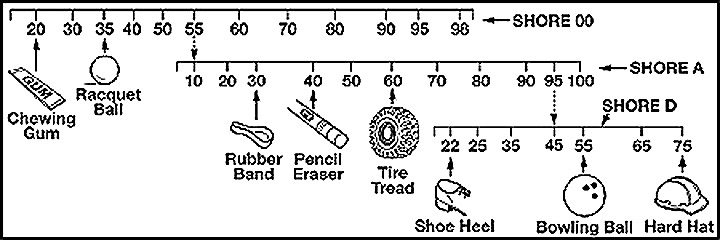
\includegraphics[width=0.85\textwidth]{imgs/shore_hardness.jpeg}
 	\caption{Shore Hardness scales, with some examples}
 \end{figure}
 
 \textit{Shore} AKA \textit{Durometer} scales are suited to measuring elastomers (i.e. rubber). Again it is important to note there are different scales. 90A is much softer than 90D durometer, although they look like they are the same on the above chart, material rated as 95A may be quite different than 45D.
 
 Elastomers are much harder to measure in other ways, and are often given ratings only by their durometer. While this is technically only a measure of hardness, it correlates reasonably well to other material properties like overall stiffness (harder being stiffer) and grip (softer being more interactive, or frictional).
 
 The thermal properties of a material are important. There are three main ones to keep in mind if you are dealing with heat:
 \begin{asparaitem}
 	\item \textit{Thermal conductivity} is how well the material transfers heat. If you're designing a heat sink, you want a high thermal conductivity.
 	\item The \textit{melting point} or \textit{glass transition temperature} are temperatures at which the material undergoes fundamental phase changes. You obviously need to make sure your part doesn't outright melt, but you should also have a bit of margin, as the phenomenon called \textit{creep} can cause parts that are at elevated temperatures to deform over time, even though below melting point.
 	\item The \textit{cefficient of thermal expansion} measures how much material expands as it heats up. If you're working with tight-tolerance equipment (or extreme temperatures), you may need to keep an eye on this.
 \end{asparaitem}
  
 Frictional characteristics and chemical interactions are very complex, and if you care about these, will require some research beyond mere datasheets.
 
 To actually get data to make material comparisons,
 \begin{asparaitem}
 	\item \href{http://www.matweb.com/search/DataSheet.aspx?MatGUID=3a2e111b27ef4e5d813bad6044b3f318&ckck=1}{\color{red}\underline{MatWeb}} has a wide range of material properties.
 	\item \href{https://www.makeitfrom.com/}{\color{red}\underline{MakeItFrom}} has a similarly wide range of materials, and includes a comparison tool to help evaluate different options.
 \end{asparaitem}
 
 % TODO: General trends / table
 % TODO: Talk about tempering & hardening, maybe?
 
 \section{Form Factors}
 
 Just because the material you want exists, doesn't mean it's widely available in the shape you want. There are a lot of different shapes that a material may be available in, and there are tradeoffs with each different form factor.
 
 \subsection{Cast from Ingnot}
 
\begin{figure}[H]
	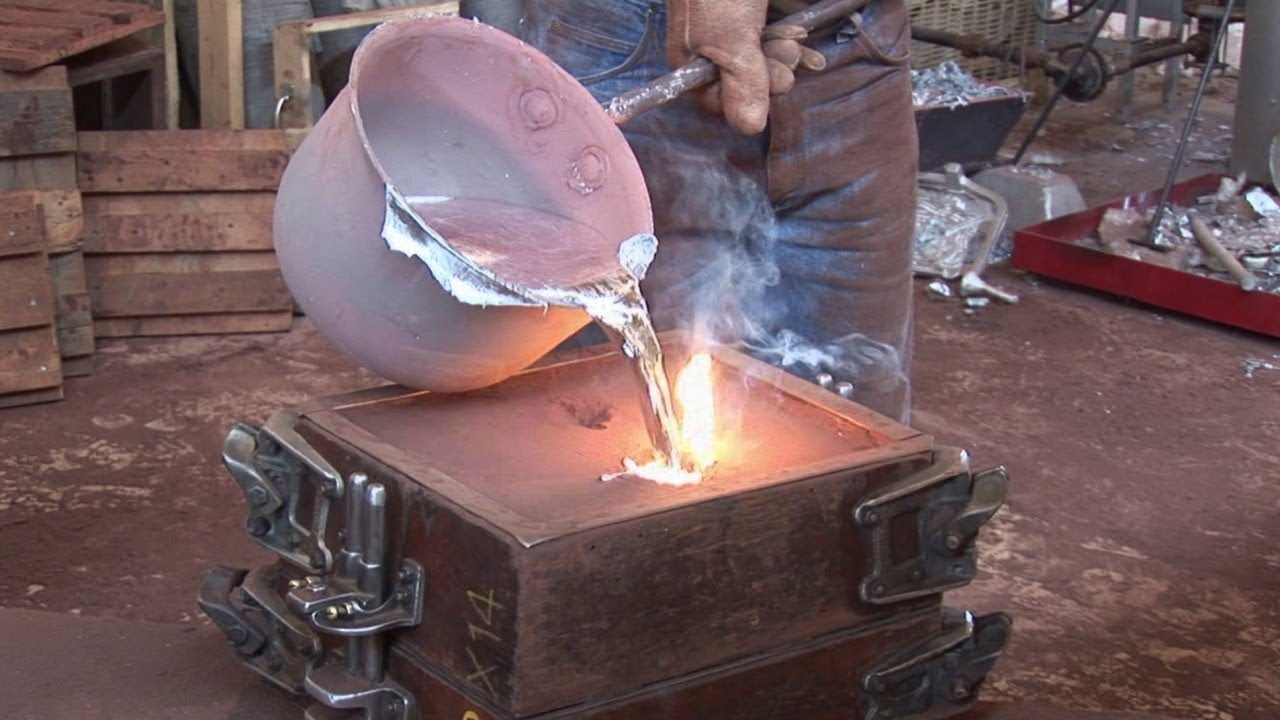
\includegraphics[width=0.55\textwidth]{imgs/casting_proc.jpeg}
	\qquad
	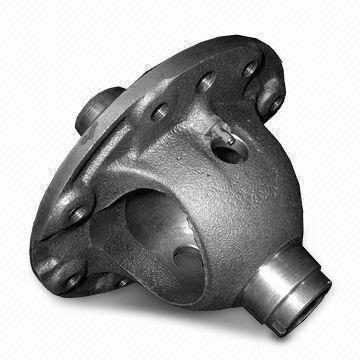
\includegraphics[width=0.3\textwidth]{imgs/casting_part.jpeg}
	\caption{Left: the casting process. Right: A cast differential housing.}
\end{figure} 
 \textit{Casting} is the process of pouring molten material into a mold to produce a complex shape. This shape isn't perfect, as the mold is usually made of sand (in order to withstand the molten metal) and the pouring process can introduce voids and imperfections, so the material properties are usually not as good. Cast parts have notably inferior material properties from billet or forged counterparts.
 
 \subsection{Billet and Plate}
 
 \begin{figure}[H]
	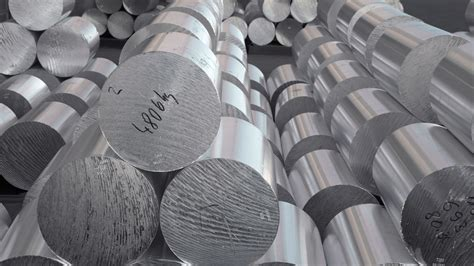
\includegraphics[width=0.6\textwidth]{imgs/billet.jpeg}
	\caption{Pieces of round billet.}
\end{figure} 
 \textit{Billet} material has been poured in a more tightly controlled environment. The resulting material is free of voids and has superior mechanical properties. You can obtain billet plate, bars, or round stock of nearly any material. This material can be held to reasonable tolerances (and by its simple-shaped nature, can be brought into exact dimension by machining quite easily).
 
 \subsection{Extrusions}
 \textit{Extruded} material has been squeezed through a die while molten, and then cooled. Think of a pasta machine. This die can be anywhere from a simple shape like a flat bar, to box tubing, to a very complicated profile with t-slots such as 80/20. Aluminum is the most common material to be extruded. Extrusions have good material properties, and can be held to tight tolerances.
 
  \begin{figure}[H]
	\centering
	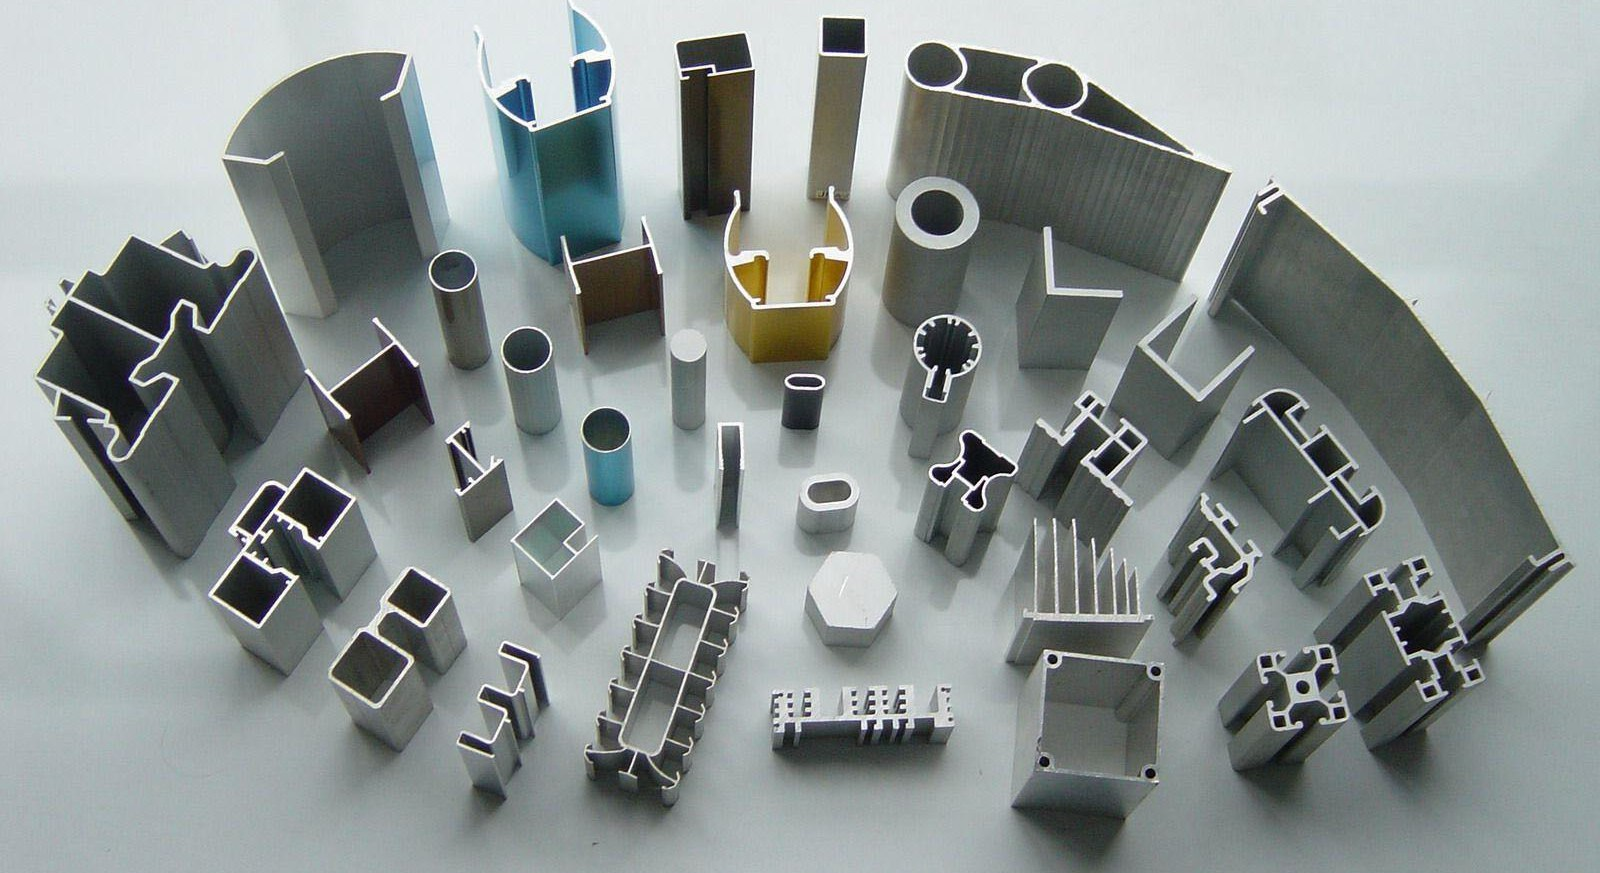
\includegraphics[width=0.8\textwidth]{imgs/extrusions.jpeg}
	
	\caption{Various Extrusions}
\end{figure}
 
 \subsection{Welded / DOM tubing}
 Steel is not easily extruded, so to make hollow shapes, must be tackled differently. Steel tubes are usually formed by taking sheet and rolling it into a tube, and then welding it together. This process leaves a weld seam which can produce odd material properties, produce dimensional issues (as when making telescoping tubes), or make manufacturing annoying (as the weld is difficult to drill through). 
 
   \begin{figure}[H]
	\centering
	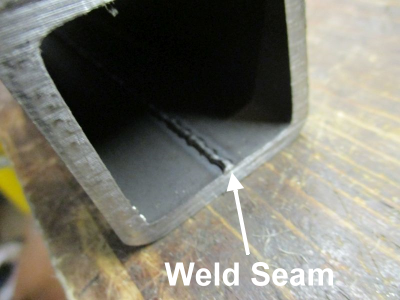
\includegraphics[width=0.4\textwidth]{imgs/welded_tube_seam.png}
	
	\caption{Weld Seam on Tubing}
\end{figure}
 
 \textit{DOM (Drawn-Over-Mandrel)} or \textit{seamless} tubing further processes this tubing to remove the inner seam and produce a product as if it were extruded. It is typically used in demanding applications such as aerospace or motorsport, as well as in components which cannot have a weld seam (such as a reciever hitch, or telescoping tubes).
 
 \subsection{Sheet}
 Material that is sold as 'sheet' rather than 'plate' usually has little-to-no straightness tolerance (in especially thin gagues, it might even be sold as rolls).
 
 \section{Manufacturing Processes}
 
 Once you have a material you like in a shape you can use, you (probably) have to cut or form it into the final shape you want. There are nearly infinite ways of doing this, but here are the most common.
 
 \subsection{Casting/Sintering/Forging}
 
 Casting, sintering, and forging are manufacturing methods which generally require a lot of tooling in order to accomplish, so are generally not suitable for quick-turnaround prototypes such as we need. Some notes, though:
 
 \begin{asparaitem}
 	\item \textit{Casting} as mentioned before, is pouring molten metal into a mold. It can produce very complex shapes (like engine blocks), but the material may end up with lots of voids.
 	\item \textit{Forging} is heating up a metal so that it can be more easily formed, though not liquid. It is then pressed between large dies to form it into the desired shape- essentially, industrialized blacksmithing. Forging can produce fairly complex shapes (like crankshafts), while preserving (and even enhancing) material properties.
 	\item \textit{Sintering} is compressing and heating powder in a mold. Also known as \textit{powder metallurgy}. This can produce somewhat simple parts with good material properties and no draft- many small gears are made this way.
 \end{asparaitem}
 
 \subsection{Machining}
 
 Machining is a broad category of processes that cut material away with a sharp tool. There are many tools that can be used to accomplish this, but there are three that are the most essential and common:
 
 \begin{figure}[H]
	\centering
	\begin{subfigure}[b]{.24\linewidth}
		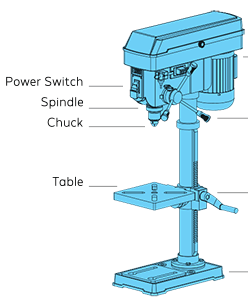
\includegraphics[width=0.95\textwidth]{imgs/drillpress.png}
		\caption{Drill press}
	\end{subfigure}	\begin{subfigure}[b]{.34\linewidth}
		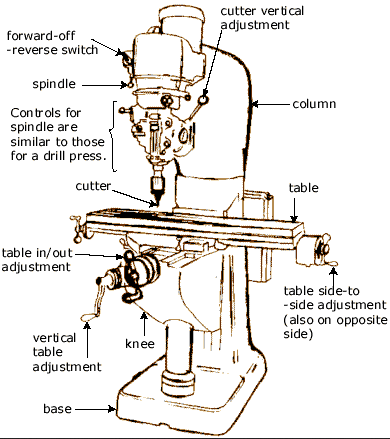
\includegraphics[width=0.95\textwidth]{imgs/mill.png}
		\caption{Milling machine}
	\end{subfigure}	\begin{subfigure}[b]{.4\linewidth}
		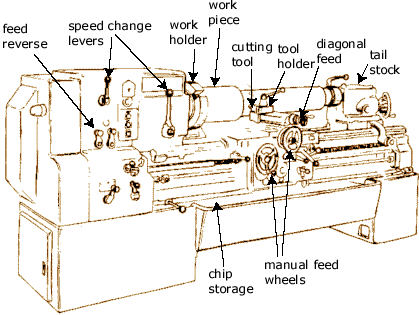
\includegraphics[width=0.95\textwidth]{imgs/lathe.png}
		\caption{Lathe}
	\end{subfigure}	
	
	\caption{The Most Common Machining Tools}
\end{figure}

 \begin{asparaenum}[a)]
 	\item A \textit{drill press} has a rotating spindle and chuck where drillbits can be inserted. Workpieces are clamped to a fixed table. The spindle can then be brought down and into the work to drill holes.
 	\item A \textit{milling machine} has a rotating spindle where drillbits and mill bits (end mills) can be inserted. Workpieces are secured to a table that moves in X, Y, and Z with respect to the spindle. \textit{Routers} operate by the same principle, but generally refer to a tool which moves much more in the X and Y than the Z, and may not be as rigid (so is more suitable to cutting sheets of plywood or foam).
 	\item A \textit{lathe} has a rotating spindle where the workpiece is held securely. Cutting tools are mounted to a carriage which moves along ways axially and radially, shaping the exterior of the work. Additionally, a tailstock can accept drill bits and other supporting devices.
 \end{asparaenum}
 
  There are lots of variations on these machines- combinations of these exist, and 4- and 5- axis mills (where the head or table tilt on the fly) also exist. They can also all be enhanced with the addition of \textit{CNC} (Computerized Numeric Control) in order to produce even more complicated shapes and/or increase productivity.
  
 These different machines can accept a wide variety of cutting implements. Here are a few of the most common to consider.
 
 \begin{figure}[H]
	\centering
	\begin{subfigure}[b]{.19\linewidth}
		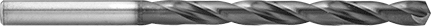
\includegraphics[width=0.95\textwidth]{imgs/drillbit.png}
		\caption{Drillbit}
	\end{subfigure} \begin{subfigure}[b]{.19\linewidth}
		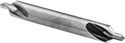
\includegraphics[width=0.95\textwidth]{imgs/centerdrill.png}
		\caption{Centerdrill}
	\end{subfigure}	\begin{subfigure}[b]{.19\linewidth}
		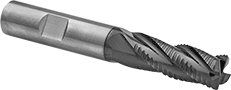
\includegraphics[width=0.95\textwidth]{imgs/endmill.png}
		\caption{End mill}
	\end{subfigure}	\begin{subfigure}[b]{.19\linewidth}
		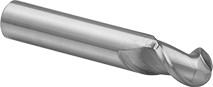
\includegraphics[width=0.95\textwidth]{imgs/ball_endmill.png}
		\caption{Ball end mill}
	\end{subfigure}\begin{subfigure}[b]{.19\linewidth}
		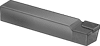
\includegraphics[width=0.95\textwidth]{imgs/lathetool.png}
		\caption{Lathe tooling}
	\end{subfigure}	
	
	\caption{Machine Tooling}
\end{figure}

 \begin{asparaenum}[a)]
 	\item \textit{Drillbits} drill holes. The spiral flutes on the outside may be sharp, but they generally aren't sharp or hard enough to actually cut metal. They work with jacobs chucks, which are designed to only transmit vertical force and torque.
 	\item \textit{Centerdrills} are used to start holes. They are short and stubby, so don't deflect much.
 	\item \textit{End mills} cut on all surfaces- they are all ground to be sharp and cut. This means they can cut on the side, and produce side loads- so they should not be put in jacobs chucks in drill presses!
 	\item \textit{Ball end mills} are an example of a more sophisticated end mill. There are many different shapes. This one enables smooth contours to be made.
 	\item \textit{Lathe tooling} comes in many different shapes and sizes. This one is a simple cutting tool that gets clamped to the toolpost and shapes the outside of the work.
 \end{asparaenum}
 
If you can consider briefly how these machines work, you can perhaps spot a few problems with your designs as you go along. Can you spot (just by the images) some issues with these parts?
 
\begin{figure}[H]
	\centering
	\begin{subfigure}[b]{.24\linewidth}
		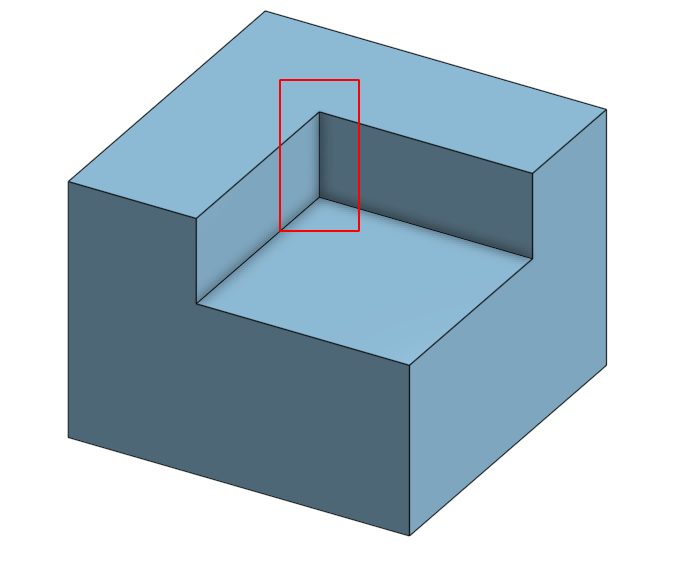
\includegraphics[width=0.9\textwidth]{imgs/nonmill_sharpins.png}
		\caption{Sharp inside corner}
	\end{subfigure}	\begin{subfigure}[b]{.24\linewidth}
		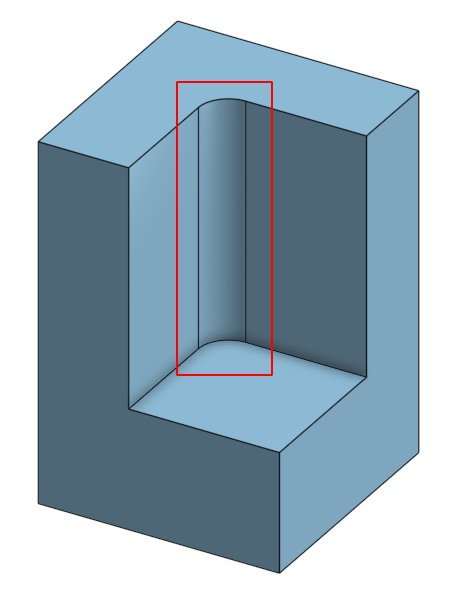
\includegraphics[width=0.9\textwidth]{imgs/nonmill_dtod.png}
		\caption{Deep radius}
	\end{subfigure}	
	
	\caption{Problematic geometries for machining}
\end{figure}

 \begin{asparaenum}[a)]
 	\item The sharp inside corner cannot be made, as it would require an infinitely small diameter tool.
 	\item The deep radius would require a very long end mill, which would not be very stiff. This radius is 0.25", and it is 2" tall; this is a ratio of depth-to-diameter of 4:1, which is a suboptimal ratio. Ideally, this ratio would be no more than 3:1.
 \end{asparaenum}
 
 \subsection{Broaching}
 
 
 \begin{figure}[H]
 	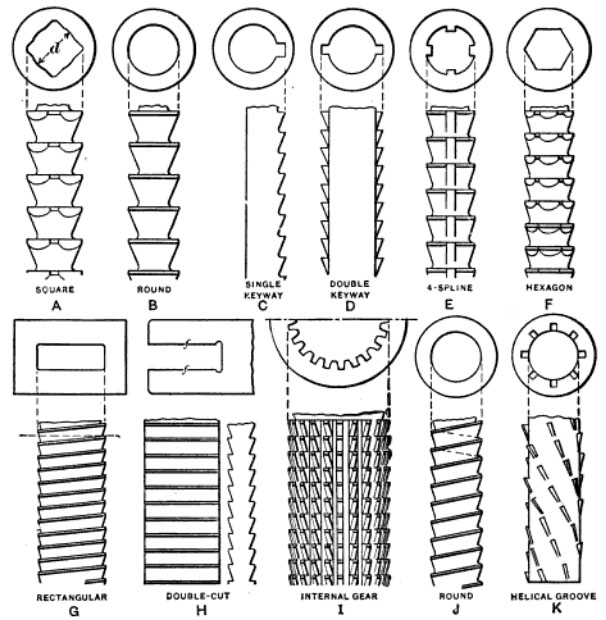
\includegraphics[width=0.6\textwidth]{imgs/broach_examples.jpeg}
 	\caption{Broach Examples}
 \end{figure}
 
 But how do we make splines, keyways, and hexes in things? Those need infinitely sharp corners, so we broach them. This is done by first drilling a hole of the appropriate diameter, and then inserting a broaching tool into the hole. The tool is then pushed through with a press. Each tooth of the broach takes off gradually more material until the final shape is achieved. Broaches are typically very expensive and relatively delicate tools.
 
 \begin{figure}[H]
 	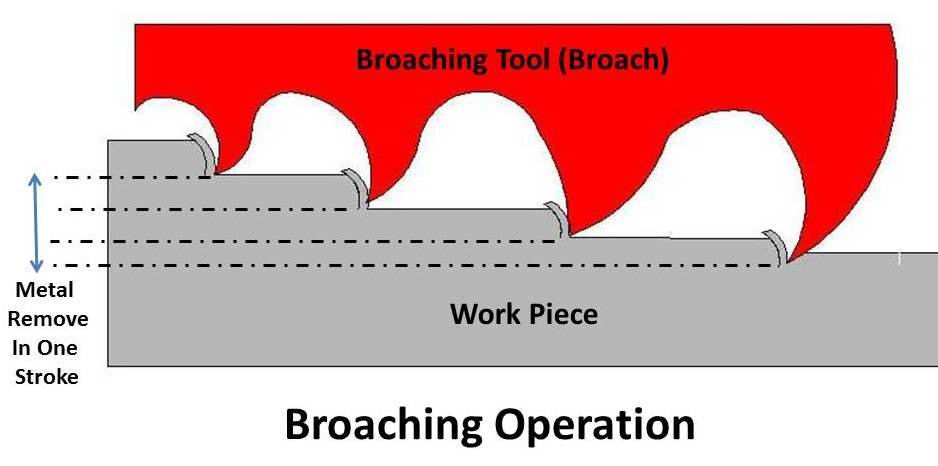
\includegraphics[width=0.7\textwidth]{imgs/broach_detail.jpeg}
 	\caption{Broach Detail}
 \end{figure}
 
 
 \subsection{Path Cutting}
 
 \textit{Path cutting} is a term I made up that encompasses any sort of 2-dimensional X/Y cutting with a thin beam. It is almost always done on a CNC-capable machine.
 
 \begin{figure}[H]
		\begin{subfigure}[b]{.24\linewidth}
			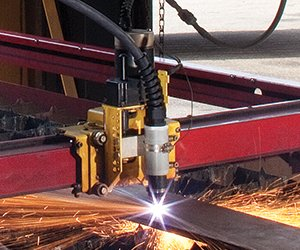
\includegraphics[width=0.9\textwidth]{imgs/plasmacut.jpeg}
			\caption{Plasma cutting}
		\end{subfigure}\begin{subfigure}[b]{.24\linewidth}
			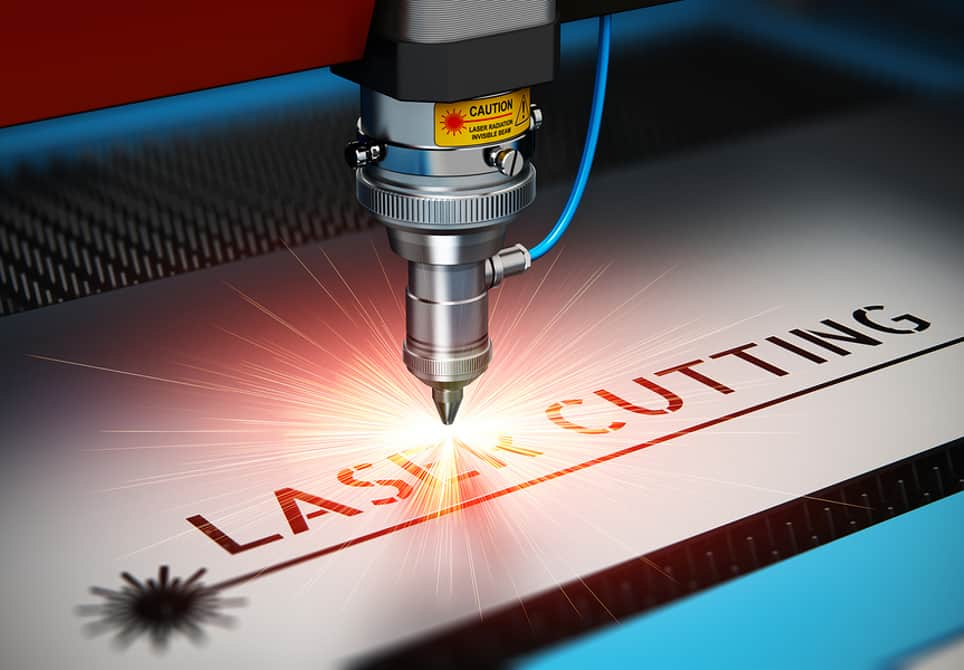
\includegraphics[width=0.9\textwidth]{imgs/lasercut.jpeg}
			\caption{Laser cutting}
		\end{subfigure}\begin{subfigure}[b]{.24\linewidth}
			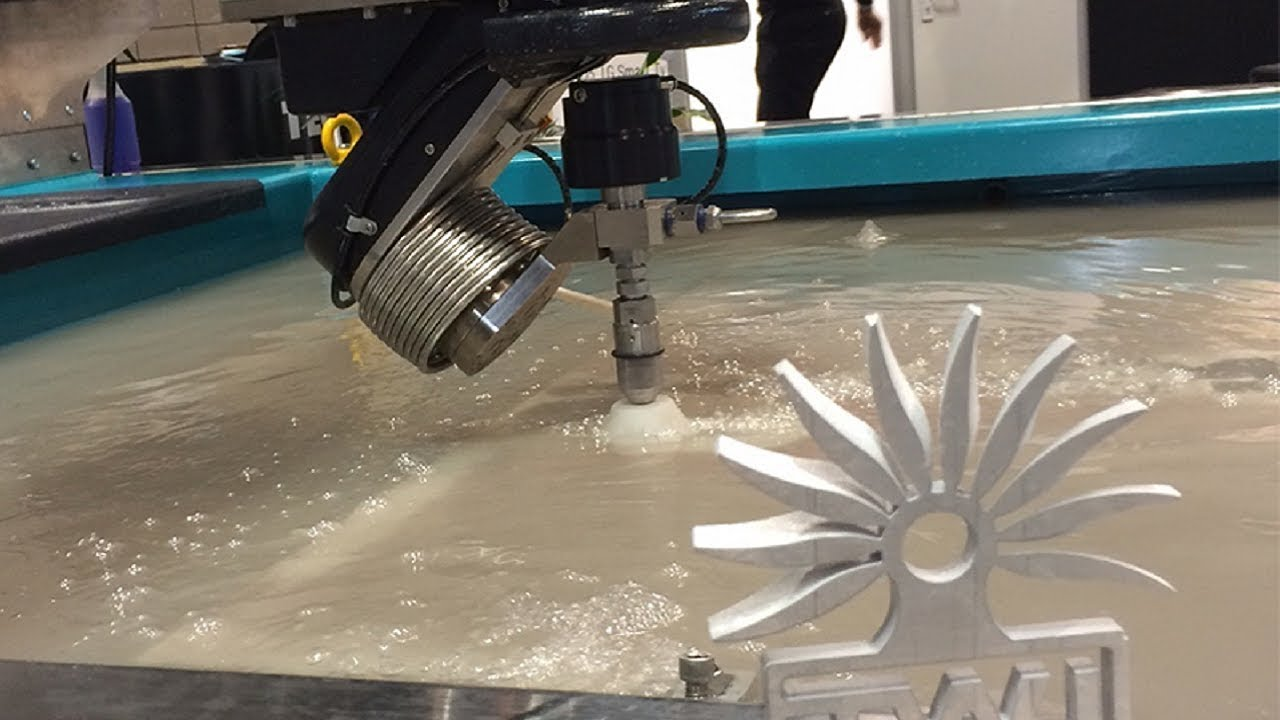
\includegraphics[width=0.9\textwidth]{imgs/waterjet.jpeg}
			\caption{Waterjet cutting}
		\end{subfigure}\begin{subfigure}[b]{.24\linewidth}
			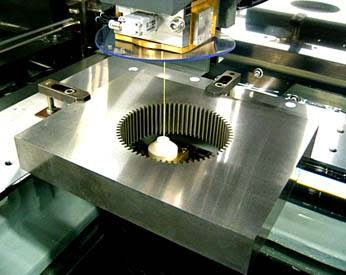
\includegraphics[width=0.9\textwidth]{imgs/edm.jpeg}
			\caption{EDM cutting}
		\end{subfigure}
	\end{figure}
 
 \begin{asparaenum}[a)]
  	\item \textit{Plasma cutters} use an arc to melt metal and pressurized air to blow it away. The tolerances are usually good for large shapes, but not for precision work.
 	\item \textit{Laser cutters} melt material with a laser and either simply vaporize it or use pressurized air to blow it away. Hobby lasers can cut some plastics and plywood, while industrial systems can cut metal. The tolerances are usually acceptable with these machines ($\pm 0.020"$).
 	\item \textit{Waterjet cutters} mix high-pressure water with garnet sand, and blast it at material, rapidly abrading it. The tolerances are usually good with this process ($\pm 0.010"$ or better).
 	\item \textit{EDMs} (electro-discharge-machines) use an electrified wire to remove material. The wire is fed through (or plunged into) material. The electrification 'zaps' away material next to the wire. The tolerances with this process can be impeccable ($\pm 0.001"$ or better). 
\end{asparaenum}
 	
 	These all allow us to overcome the depth-to-diamter ratio imposed by milling, and can sometimes be much quicker setup than traditional machining, though they all come with their own drawbacks.
 
 \begin{figure}[H] \centering
 	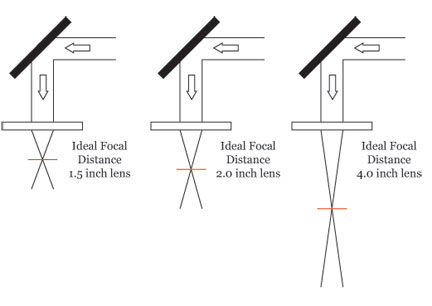
\includegraphics[width=0.5\textwidth]{imgs/lasercut_focus.jpeg}
 	\caption{Focal properties of a lasercutter's beam.}
 \end{figure}
 
  The first limitation is the width of the beam. Since a finite-ly sized beam muse be used, infinitely sharp interior corners cannot be made.
 
 \begin{figure}[H] \centering
 	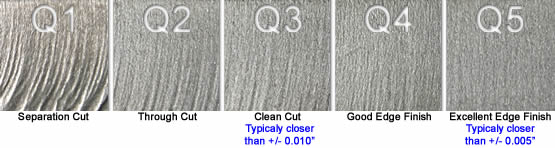
\includegraphics[width=0.9\textwidth]{imgs/waterjet_draft.jpeg}
 	\caption{Draft and surface quality samples on a waterjet with different settings.}
 \end{figure}
 
  The next consideration that must be made is draft. Laser-cutters typically have a point in the thickness where the beam is focused to. This means that the laser doesn't cut a line in its cross-section, but rather an X. Thus the resulting shape is two-dimensional. With a waterjet or plasma cutter, the draft grows exponentially. This may be acceptable, or require further post-machining to bring it into specification.
 
 Draft (and power) also limits how thick of material can feasibly be cut with these processes, although EDM can cut extremely thick materials compared to the other processes.
 
 \subsection{Sheet Forming}
 
 Sheet forming is a versatile process of making parts from, well, sheet. Sheet may be cut either with a stamping operation, or with a path-cutting operation to form a blank. This blank can then be loaded in and undergo one of several processes.
 
 	\begin{figure}[H]
		\centering
		\begin{subfigure}[b]{.24\linewidth}
			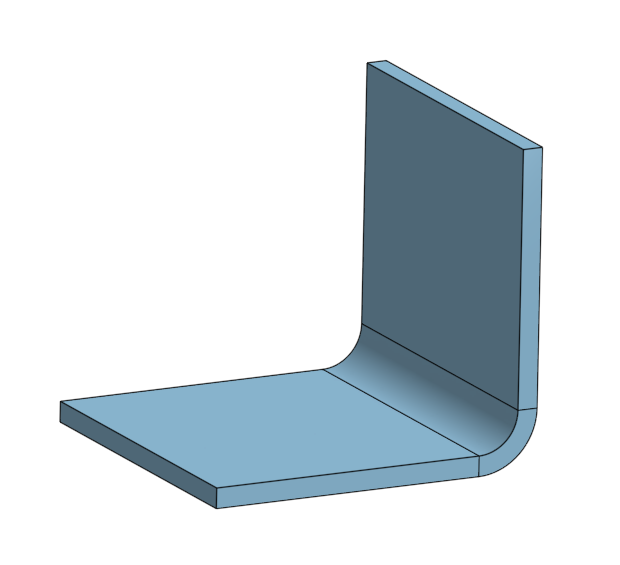
\includegraphics[width=0.9\textwidth]{imgs/sheet_bend.png}
			\caption{Bend}
		\end{subfigure}\begin{subfigure}[b]{.24\linewidth}
			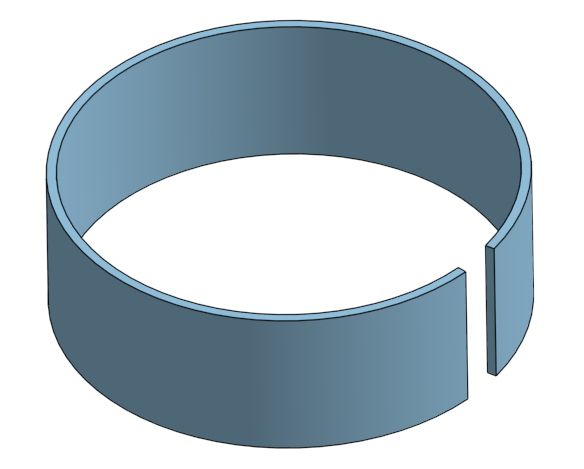
\includegraphics[width=0.9\textwidth]{imgs/sheet_roll.png}
			\caption{Rolling}
		\end{subfigure}\begin{subfigure}[b]{.24\linewidth}
			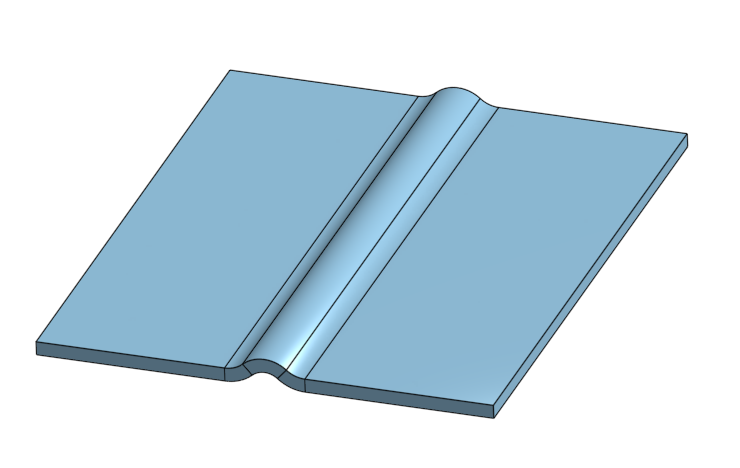
\includegraphics[width=0.9\textwidth]{imgs/sheet_beadroll.png}
			\caption{Bead Rolling}
		\end{subfigure}\begin{subfigure}[b]{.24\linewidth}
			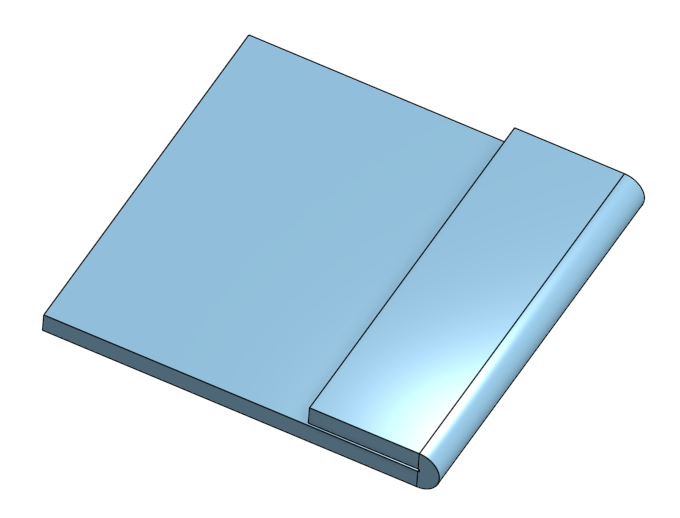
\includegraphics[width=0.9\textwidth]{imgs/sheet_hem.png}
			\caption{Hemming}
		\end{subfigure}
		\caption{Rudimentary sheetmetal operations.}
	\end{figure} 
 
 \begin{asparaenum}[a)]
 	\item Simple \textit{bends} can be made on a linear portion of the flat pattern. This can be done with a finger bender, press brake, or (in a pinch) a vise with a hammer.
 	\item Flat portions of material can be \textit{rolled} into an arc, or even full circle.
 	\item \textit{Bead rolling} can be done on any portion of a part to provide additional stiffness.	
 	\item \textit{Hemming} provides a smooth, radiused outer corner and some additional stiffness. First, a bend is made, and then it is bent all the way to 180 degrees. This can be done with a finger bender or press brake, and additional clamping to finish the hem.
 	\end{asparaenum}
 	
 	Most CAD packages have tools to design parts made with sheetmetal. You can draw up the bent part, and then the CAD package will determine how to 'unfold' and produce a flat pattern that can be cut out.
 	
 	These operations are typically done with metal, but nothing prevents you from doing it with plastic. Polycarbonate can be bent like sheetmetal. Polypropylene, polycarbonate, acrylic, and PETG amongst others can also be heated (i.e. with a heat gun) and then bent by hand.
 	
 	\subsection{Welding and Brazing}
 	
 	Welding and brazing are very important manufacturing methods. They enable large, complex structures to be made from smaller simple ones, without fasteners that might fail. However, it can be quite time consuming, requires time consuming labor, and creates non-servicable structures.
 	
 	\begin{figure}[H]
		\centering
		\begin{subfigure}[b]{.24\linewidth}
			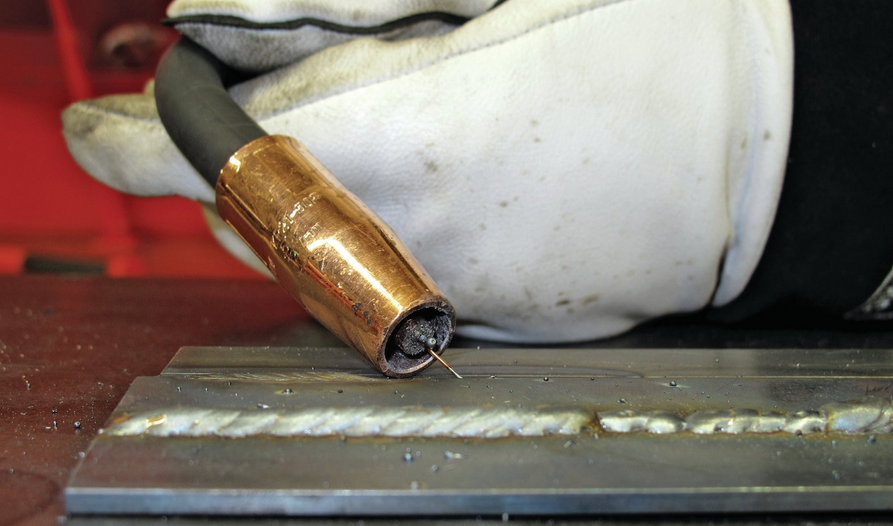
\includegraphics[width=0.9\textwidth]{imgs/mig.png}
			\caption{MIG}
		\end{subfigure}\begin{subfigure}[b]{.24\linewidth}
			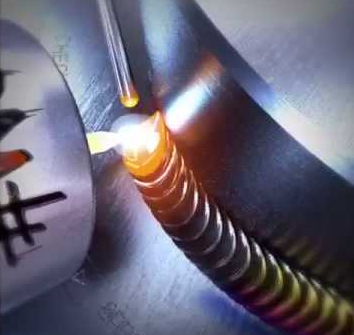
\includegraphics[width=0.9\textwidth]{imgs/tig.png}
			\caption{TIG}
		\end{subfigure}\begin{subfigure}[b]{.24\linewidth}
			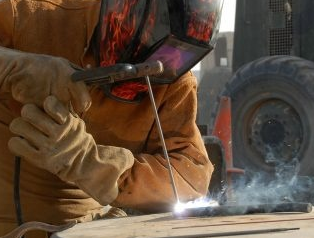
\includegraphics[width=0.9\textwidth]{imgs/arcweld.png}
			\caption{Stick/Arc Welding}
		\end{subfigure}\begin{subfigure}[b]{.24\linewidth}
			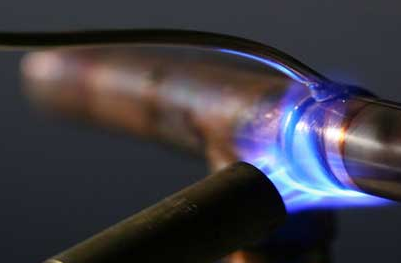
\includegraphics[width=0.9\textwidth]{imgs/braze.png}
			\caption{Brazing}
		\end{subfigure}
		\caption{Various welding/brazing technologies.}
	\end{figure}
 	
 	\begin{asparaenum}[a)]
 		\item \textit{MIG} (Metal-Inert-Gas) welding uses an electric arc between filler wire and the workpiece, which melts both the wire and the workpiece. The arc is shielded by inert (or semi-active) gas to control chemical reactions. The wire is advanced at a constant rate into the workpiece. This is the easiest method to learn, but provides the least amount of control, and has the lowest capacity for superior results.
 		
 		\item \textit{TIG} (Tungsten-Inert-Gas) welding uses an electric arc between a fixed tungsten rod and the workpiece, melting the work but not the tungsten. The arc is shielded by inert gas to eliminate chemical reactions. Filler rod is advanced manually and separately into the molten work. This method is much harder to learn, but provides the most amount of control, with the highest capacity for superior results.
 		
 		\item \textit{Stick} (or Arc) welding uses an electric arc between a rod containing flux and filler metal and the workpiece, melting both the rod and the workpiece.. The arc is shielded by the vaporizing flux. This method is hard to learn, but provides good control, and works best outdoors, so is quite common in the construction and pipeline industries.
 		
 		\item In \textit{brazing}, heat is generated (either by a TIG torch, or a flame torch) and directed at the work, but not enough to melt the work. Brazing material, which will melt at this surface temperature, is fed onto the work, melting and flowing across it. As it solidifies, it adheres to the base metal.
 		
 	\end{asparaenum}
 		
	\section{Fasteners}
	So you've made some parts, now it's time to put them together. How are you going to do it? CAD constraints won't help you now! You need real fasteners!
	
	\subsection{Pins}
	The simplest fastener is a pin. Pins prevent holes in plates from shearing past each other, by putting all of the load through the pin. There are a couple different flavors that let you do different things.
	
	Quick pins allow users to easily make adjustments or reconfigurations to equipment. They are easily insertable/removable, usually without any special tools.
	
	\begin{figure}[H]
		\centering
		\begin{subfigure}[b]{.32\linewidth}
			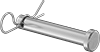
\includegraphics[width=0.7\textwidth]{imgs/cpin.png}
			\caption{Clevis pin}
		\end{subfigure}\begin{subfigure}[b]{.32\linewidth}
			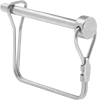
\includegraphics[width=0.7\textwidth]{imgs/wlpin.png}
			\caption{Wire-locking pin}
		\end{subfigure}\begin{subfigure}[b]{.32\linewidth}
			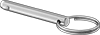
\includegraphics[width=0.7\textwidth]{imgs/bdpin.png}
			\caption{Ball-detent pin}
		\end{subfigure}
		\caption{Various quick-removal pins.}
	\end{figure}
	
	\begin{asparaenum}[a)]
		\item \textit{Clevis pins} are loose tolerance pins which have a hole for a locking (R-shaped) pin or wire to go through.
		\item \textit{Wire-Locking pins} serve the same purpose as clevis pins, but use a spring-loaded wire to keep the pin captive.
		\item \textit{Ball-Detent pins} serve the same purpose as clevis pins, but use a spring-loaded ball detent to keep the pin captive. These can be pulled/pushed in without and additional steps.
	\end{asparaenum}
	
	
	Precision pins serve a nearly opposite purpose- they are permanent instalations, but provide extremely tight tolerances when used right. They allow for installation/detachment of components with high repeatability in locational positioning. It's not uncommon to see precision equipment register together with pins, and then be bolted together in addition to the pins. Pins also can provide higher load transferral since they do not have the stress concentrators that bolts do.
	
	\begin{figure}[H]
		\centering
		\begin{subfigure}[b]{.24\linewidth}
			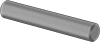
\includegraphics[width=0.7\textwidth]{imgs/dpin.png}
			\caption{Dowel pin}
		\end{subfigure}\begin{subfigure}[b]{.24\linewidth}
			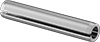
\includegraphics[width=0.7\textwidth]{imgs/spin.png}
			\caption{Spring pin}
		\end{subfigure}\begin{subfigure}[b]{.24\linewidth}
			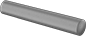
\includegraphics[width=0.7\textwidth]{imgs/tpin.png}
			\caption{Taper pin}
		\end{subfigure}\begin{subfigure}[b]{.24\linewidth}
			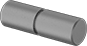
\includegraphics[width=0.7\textwidth]{imgs/shpin.png}
			\caption{Shear pin}
		\end{subfigure}
		\caption{Various precision pins.}
	\end{figure}
	
	\begin{asparaenum}[a)]
		\item \textit{Dowel pins} are tight-tolerance. They are typically pressed into one part's hole, and with a loose fit on another mating part.
		\item \textit{Spring pins} are formed from coiled metal, intended to be pressed in like a dowel pin, but have some give to them so can be used with looser-tolerance holes.
		\item \textit{Taper/scotch pins} are like dowel pins, but they are slightly tapered, so they wedge into multiple parts like a nail.
		\item \textit{Shear pins} are specifically designed to fail at a specified load, which prevents damage to equipment down-the-line.
	\end{asparaenum}
	
	\subsection{Threads}
	
	Threaded fasteners (bolts, nuts, and screws) are a ubiquitous solution. There's an age old question of what is a 'screw' versus a 'bolt' and the answer is merely in application- if it goes into a nut, it's a bolt. Otherwise, it's a screw. So, anything said about screws is true of bolts and vise-versa. Threaded fasteners are denoted by:
	
	% TODO: NICE GRAPHIC
	
	\begin{asparaitem}
		\item The major diameter of the thread.
		\item The thread pitch, or threads-per-inch. Metric bolts are specced by the pitch (a M5x0.8 has 0.8mm between each thread crest). English bolts are specced by the number of threads in an inch (a 1/4"-20 has 20 threads per inch). Even among the same diameter, bolts can have different pitches. For instance, a 1/4"-28 is fine thread, and a 1/4"-20 is coarse thread.
		\item The thread length - the bolt might be threaded fully, or only partially.
		\item The handedness of the thread - most threads are right handed (meaning turning them in a clockwise fashion will make them move away) unless specified as left-handed.
		\item The grade or class - this refers to the strength of the material. English bolts are specified by "grade", and metric bolts by "class". Bolts (usually) have head markings that reflect the material. Grade and class are only for steel, though- other materials have more exotic standards.
	\end{asparaitem}
	
	There are many different types of bolts out there.
	
	\begin{figure}[H]
		\centering
		\begin{subfigure}[b]{.24\linewidth}
			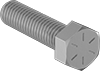
\includegraphics[width=0.7\textwidth]{imgs/hhcs.png}
			\caption{External drive}
		\end{subfigure}\begin{subfigure}[b]{.24\linewidth}
			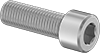
\includegraphics[width=0.7\textwidth]{imgs/shcs.png}
			\caption{Socket head}
		\end{subfigure}\begin{subfigure}[b]{.24\linewidth}
			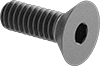
\includegraphics[width=0.7\textwidth]{imgs/fhcs.png}
			\caption{Flathead}
		\end{subfigure}\begin{subfigure}[b]{.24\linewidth}
			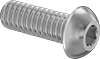
\includegraphics[width=0.7\textwidth]{imgs/bhcs.png}
			\caption{Button head}
		\end{subfigure}
		
		\begin{subfigure}[b]{.24\linewidth}
			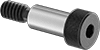
\includegraphics[width=0.7\textwidth]{imgs/shoulderscrew.png}
			\caption{Shoulder screw}
		\end{subfigure}\begin{subfigure}[b]{.24\linewidth}
			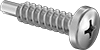
\includegraphics[width=0.7\textwidth]{imgs/stscrew.png}
			\caption{Self-tapping screw}
		\end{subfigure}\begin{subfigure}[b]{.24\linewidth}
			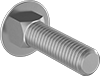
\includegraphics[width=0.7\textwidth]{imgs/carriagebolt.png}
			\caption{Carriage bolt}
		\end{subfigure}\begin{subfigure}[b]{.24\linewidth}
			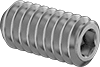
\includegraphics[width=0.7\textwidth]{imgs/grubscrew.png}
			\caption{Grub or set screw}
		\end{subfigure}
		\caption{Various screws / bolts.}
	\end{figure}
	
	\begin{asparaenum}[a)]
		\item \textit{External drive} bolts are good when only side-access is possible, or a cheap solution is needed. The most common example is a hex-head bolt, though pentagon-, external-torx-, and square- heads exist.
		\item \textit{Socket head} bolts are preferred. They can be installed in deep wells and have a compact head profile.
		\item \textit{Flat head} screws need to be installed into holes that have been countersunk to the same angle as the head of the screw. They allow for a flush, smooth installation. However, they have a smaller hex than socket heads of the same thread diameter. This makes them more prone to stripping the head out.
		\item \textit{Button head} screws provide a smooth surface without the need to countersink the surface. They still have a smaller-diameter hex than socket-heads, though, so are generally unpreferred.
		\item \textit{Shoulder screws} are special-use screws. The shoulder (unthreaded) portion is precision ground and usually a larger diameter than the thread. This allos them to be used as pins or pivot points.
		\item \textit{Self-tapping screws} have specially formed tips based on what material they are designed to tap into. They thread into material directly; a tap is not required to form threads, and in plastic and wood, are generally stronger.
		\item \textit{Carriage bolts} have a rounded head without any means of being driven externally. Instead, the square portion sitting under the thread mates with the material it bolts together (either a plate with the corresponding female portion, or a soft material like wood conforms to the square). \textit{Plow bolts} are the same principle, but are flat-headed.
		\item \textit{Set screws} (often called \textit{grub screws}) are used to lock down on another piece of material. Commonly seen to secure hubs to shafts. They have very small hexes relative to their thread diameter and are notorious for stripping out.
	\end{asparaenum}
	
	There are a lot of different head types that can be put on these bolts as well. 
	
	\begin{figure}[H]
		\centering
		\begin{subfigure}[b]{.15\linewidth}
			
\includegraphics[width=0.7\textwidth]{imgs/head_ext_hex.png}
			\caption{External hex}
		\end{subfigure}\begin{subfigure}[b]{.15\linewidth}
			
\includegraphics[width=0.7\textwidth]{imgs/head_hex.png}
			\caption{Socket hex}
		\end{subfigure}\begin{subfigure}[b]{.15\linewidth}
			
\includegraphics[width=0.7\textwidth]{imgs/head_slot.png}
			\caption{Flathead}
		\end{subfigure}\begin{subfigure}[b]{.15\linewidth}
			\includegraphics[width=0.7\textwidth]{imgs/head_phil.png}
			\caption{Phillips}
		\end{subfigure}\begin{subfigure}[b]{.15\linewidth}
			\includegraphics[width=0.7\textwidth]{imgs/head_torx.png}
			\caption{Torx}
		\end{subfigure}\begin{subfigure}[b]{.15\linewidth}
			\includegraphics[width=0.7\textwidth]{imgs/head_robertson.png}
			\caption{Robertson}
		\end{subfigure}
		\caption{Common drive types on engineering fasteners.}
	\end{figure}
	
	\begin{asparaenum}[a)]
		\item \textit{External hex} is very robust, although prefferred only when side access is available as it has a large profile.
		\item \textit{Socket hex} has become an industry preferred head, very easy to access from head-on or in a deep pocket.
		\item \textit{Flathead} is an unpreferred drive type; it is very easy to have driver fall out while using, and the torque-transferring capacity is quite low.
		\item \textit{Phillips} heads are very much unpreferred as they are very easy to cam out (in fact, they were designed to do so as a means of limiting the installation torque). When driving a phillips screw, apply inward pressure, and make sure the proper size driver is selected (it should fit nicely).
		\item \textit{Torx} is a preferred drive method, but more expensive and the tools to use it are less common. Very difficult to strip out. When using button-head or flat-head screws, if a torx variant is available, it can be wise to opt for it as the torque-transferring capacity is higher.
		\item \textit{Robertson} or square drive is somewhat preferred, but not common. Usually found only in wood screws.
	\end{asparaenum}
	
	
	\begin{figure}[H]
		\includegraphics[width=0.5\textwidth]{imgs/bolt_preload.png}
		\caption{Aspects of a bolted joint.}
		 \label{fig:bolted_joint} 
	\end{figure}
	
	When you tighten a screw to a torque, this not only prevents the nut from falling off, but clamps the parts together. This clamping force that is imparted upon installation is \textit{preload}. Preload is very important in threaded joints. For shear loads as illustrated in Figure \ref{fig:bolted_joint}, the load is best carried by the friction inbetween plates rather than shearing the pin itself, since the load is distributed across a larger area. For joints that seal against pressures, preload is imperative as it prevents separation under pressure.
	
	The preload depends both on how much torque is applied to the fastener, and the pitch of the thread. A finer-pitched screw will impart greater preload. Finer-pitched screws also have the benefit of an increased core (minor) diameter, so greater strength in shear.
	
	Spreading the load across the greater area increases rigidity and decreases backlash, egg-out, and strength. However, too much torque can dig the head of the bolt/screw into the underlying material, especially if it is soft (like plastic, or even aluminum). As such, care not to overtorque, or a washer may be needed.
	
	\begin{figure}[H]
		\centering
		\begin{subfigure}[b]{.24\linewidth}
			\includegraphics[width=0.7\textwidth]{imgs/plainwasher.png}
			\caption{Plain washer}
		\end{subfigure}\begin{subfigure}[b]{.24\linewidth}
			\includegraphics[width=0.7\textwidth]{imgs/machinewasher.png}
			\caption{Machine washer}
		\end{subfigure}\begin{subfigure}[b]{.24\linewidth}
			\includegraphics[width=0.7\textwidth]{imgs/fenderwasher.png}
			\caption{Fender washer}
		\end{subfigure}
		\caption{Plain washers of differring sizes}
	\end{figure}
	
	Bolts thread into nuts, which can be replaced if they strip out. But if the material a screw threads into strips, then that whole piece will need to be replaced or repaired- which can be even more costly. There are some considerations that can be made to ensure success when using integral threads. The first is to make sure to use coarse (not fine) threads in soft materials like aluminum or plastic. Another option is to use thread inserts.
	
	\begin{figure}[H]
		\centering
		\begin{subfigure}[b]{.24\linewidth}
			\includegraphics[width=0.5\textwidth]{imgs/helicoil.png}
			\caption{Helicoil}
		\end{subfigure}\begin{subfigure}[b]{.24\linewidth}
			\includegraphics[width=0.5\textwidth]{imgs/tanglock.png}
			\caption{Tang-lock insert}
		\end{subfigure}\begin{subfigure}[b]{.24\linewidth}
			\includegraphics[width=0.5\textwidth]{imgs/rivnut.png}
			\caption{Rivnut}
		\end{subfigure}\begin{subfigure}[b]{.24\linewidth}
			\includegraphics[width=0.5\textwidth]{imgs/pemnut.png}
			\caption{PEM nut}
		\end{subfigure}
		
		\begin{subfigure}[b]{.24\linewidth}
			\includegraphics[width=0.5\textwidth]{imgs/heatset.png}
			\caption{Heat-set insert}
		\end{subfigure}\begin{subfigure}[b]{.24\linewidth}
			\includegraphics[width=0.5\textwidth]{imgs/teenut.png}
			\caption{Tee nut}
		\end{subfigure}\begin{subfigure}[b]{.24\linewidth}
			\includegraphics[width=0.5\textwidth]{imgs/woodsti.png}
			\caption{Wood tapping insert}
		\end{subfigure}
		\caption{Various threaded inserts}
	\end{figure}
	
	\begin{asparaenum}[a)]
		\item \textit{Helicoils} can be installed after a thread strips out, or before it does preventatively. They are a coiled piece of metal formed like threads.
		\item \textit{Tang-lock inserts} work much like helicoils, but are solid-bodied rather than coiled, and have locking tangs that can be hammered down on installation to make sure the insert doesn't back out.
		\item \textit{Rivnuts} (rivet nuts) can be installed into holes in thin metal to provide ample threads for fastening. They work much like rivets (more on those later), but need a special tool.
		\item \textit{PEM nuts} serve the same purpose as rivnuts, but are simply pressed into the sheet they are to be installed in.
		\item \textit{Heat-set inserts} are for plastic. They are instaled by heating them up with a soldering iron and pressing them into thermoplastic. An excellent addition to 3D prints.
		\item \textit{Tee nuts} are meant to be pressed into wood, much like a PEM nut. The large flange prevents tear-out and helps distribute load in soft wood.
		\item \textit{Wood tapping inserts} are much like tang-lock inserts, but with larger wings suitable for wood.
	\end{asparaenum}
	
	Threaded joints have one big weakness, and that is their subsceptibility to vibration. There are many solutions to try and combat this.
	
	\begin{figure}[H]
		\centering
		\begin{subfigure}[b]{.24\linewidth}
			\includegraphics[width=0.8\textwidth]{imgs/lockwire.png}
			\caption{Safety/lock wire}
		\end{subfigure}\begin{subfigure}[b]{.24\linewidth}
			\includegraphics[width=0.8\textwidth]{imgs/threadlocker.jpeg}
			\caption{Threadlocker}
		\end{subfigure}\begin{subfigure}[b]{.24\linewidth}
			\includegraphics[width=0.5\textwidth]{imgs/nylock.png}
			\caption{Nylock nut}
		\end{subfigure}\begin{subfigure}[b]{.24\linewidth}
			\includegraphics[width=0.7\textwidth]{imgs/kaynut.png}
			\caption{Kay/jet nut}
		\end{subfigure}
		
		\begin{subfigure}[b]{.24\linewidth}
			\includegraphics[width=0.5\textwidth]{imgs/jamnut.png}
			\caption{Jam nut}
		\end{subfigure}\begin{subfigure}[b]{.24\linewidth}
			\includegraphics[width=0.5\textwidth]{imgs/nordlock.png}
			\caption{Nordlock washer}
		\end{subfigure}\begin{subfigure}[b]{.24\linewidth}
			\includegraphics[width=0.5\textwidth]{imgs/splitlock.png}
			\caption{Split lock washer}
		\end{subfigure}\begin{subfigure}[b]{.24\linewidth}
			\includegraphics[width=0.5\textwidth]{imgs/castlenut.png}
			\caption{Castle nut}
		\end{subfigure}
		\caption{Thread locking strategies.}
	\end{figure}
	
	\begin{asparaenum}[a)]
		\item Lock wire requires tedious installation and bolts with cross-drilled holes to feed the stainless steel wire through. That said, when it is installed properly, it is virtually failure-proof, and as such is the standard in many aerospace and motorsport applications. 
		\item Threadlocker (sometimes referred to by the brand name Loctite) comes in various different strengths and can be used on metal-on-metal contact. It's basically long-cure, specially formulated superglue. However, it does attack many plastics, so be careful! It also requires time to cure to full strength, so is not an instant fix, but must be premeditated.
		\item Nylock nuts have a nylon patch that deforms when the threads pass through it. The nut should be installed metal-side first, nylon-side last. These are limited use (<50 uses).
		\item Kay/Jet nuts (metal locknuts) work on the same idea as nylock nuts, but in this case, the nut is deformed and interferes with the thread. It is quite difficult to thread into these nuts. These are extremely limited use (<5 uses) but will work in extreme temperatures, unlike nylocks.
		\item Jam Nuts are simply a second nut jammed up against the first nut. This enables easy adjustment, but is not a very positive way of locking something in place.
		\item Nordlock washers are special ratcheting washers which prevent loosening when properly torqued. There are many different types of locking washers.
		\item Split lock washers are cheap washers which arguably do not actually prevent loosening.
		\item Castle nuts are nuts with slots through which a pin can be fed, locking the nut to the bolt it is secured to. A very robust method.
	\end{asparaenum}
	
	\subsection{Rivets}
	
	Pop rivets are a light and cheap method of fastening. However, they require a special gun and are one-time use. They must be drilled out in order to remove them. They are weaker than bolts, so more must be used, but overall, they are a lighter option. Installation is also more picky than bolting. However, they can still be a time-saver over bolts (when disassembly is not a factor).
	
	Rivets are specified by diameter and 'grip length'; the amount of material sandwiched together they can grip. Rivets should be installed to close-fit holes, straight, and with the plates already pulled together.
	
	\begin{figure}[H] \centering
		\includegraphics[width=0.9\textwidth]{imgs/rivet_install.jpeg}
		\caption{Left: Process of Rivet Installation. Right: Diagnosing rivet failures.}
	\end{figure}
	
	Hot rivets are a very different animal than pop rivets. These require very specialized equipment, and work by heating up a rivet to molten temperature, inserting it through the hole to be secured, and hammering it so it expands and mushrooms out on both sides. As the rivet cools, it shrinks further, creating an incredibly robust and secure connection.	
	
	\subsection{Shaft Retention}
	
	Retaining rings are used to constrain objects along a shaft.
	
	\begin{figure}[H]
		\centering
		\includegraphics[width=0.45\textwidth]{imgs/shaft_snapringgroove.png}
		\includegraphics[width=0.45\textwidth]{imgs/snapringtool.jpeg}
		\caption{Left: Shaft with groove for retaining ring. Right: Snap ring pliers.}
	\end{figure}
	
	\begin{figure}[H]
		\centering
		\begin{subfigure}[b]{.24\linewidth}
			\includegraphics[width=0.6\textwidth]{imgs/shaftcollar.png}
			\caption{Shaft Collar}
		\end{subfigure}
		\begin{subfigure}[b]{.24\linewidth}
			\includegraphics[width=0.7\textwidth]{imgs/pushonring.png}
			\caption{Push-On Ring}
		\end{subfigure}
		\begin{subfigure}[b]{.24\linewidth}
			\includegraphics[width=0.7\textwidth]{imgs/eclip.png}
			\caption{E-Clip}
		\end{subfigure}
		\begin{subfigure}[b]{.24\linewidth}
			\includegraphics[width=0.7\textwidth]{imgs/ext_snapring.png}
			\caption{External Snap Ring}
		\end{subfigure}
		\begin{subfigure}[b]{.24\linewidth}
			\includegraphics[width=0.7\textwidth]{imgs/int_snapring.png}
			\caption{Internal Snap Ring}
		\end{subfigure}
		\begin{subfigure}[b]{.24\linewidth}
			\includegraphics[width=0.7\textwidth]{imgs/spiralring.png}
			\caption{Spiral Ring}
		\end{subfigure}\begin{subfigure}[b]{.24\linewidth}
			\includegraphics[width=0.7\textwidth]{imgs/circlip.png}
			\caption{Circlip}
		\end{subfigure}
		\caption{Shaft Retaining Technologies}
	\end{figure}
	
	
	\begin{asparaenum}[a)]
		\item \textit{Shaft collars} are heavy, high-profile, but easily removable and adjustable. They come in different bore shapes (hex, round, keyed). They come in two-piece and one-piece varieties.
		\item \textit{Push-on rings} are pushed onto shafts (no groove needed) and (ideally) ratchet on, never coming off.
		\item \textit{E-clips} can be pushed radially into a groove. They are aided by the use of a snap-ring tool to splay them apart, but it is not necessary. They can be installed without passing the clip over the end of a shaft.
		\item \textit{External snap rings} are expanded by a snap-ring tool, and installed over the groove of a shaft.
		\item \textit{Internal snap rings} are compressed by a snap-ring tool, and installed into the groove of a housing.
		\item \textit{Spiral rings} are wound into grooves. They're annoying and rare.
		\item \textit{Circlips} are very stiff, low-profile retaining clips intended for permanent installation.

	\end{asparaenum}
	
	When working with expanding rings, it is very important to not over-extend them on installation. It is very easy to over-extend and damage the rings (leading to successful installation, but potential for the ring to fall off later during use) if expanded much more than is necessary to feed them over the shaft.
	
	\subsection{Adhesives}
	
	Adhesives are useful from time to time.
	
	\begin{asparaenum}[a)]
		\item Retaining compound (e.g. Loctite Green) is meant to bond bearings to their housings, and is very good at it.
		\item Epoxies are two-part adhesives that are mixed immediately prior to application. They can cure quickly.
		\item Cryanacrolate (superglue) adhesives are good for many plastics. Loctite has a good design/test guide for different plastic/glue combinations.
		\item Tapes can be quite useful. Good duct tape and gaffers tape can be used for high-fidelity prototyping and quick fixes.
		\item Pressure-sensitive tape (e.g. 3M VHB) can be incredibly strong. Follow manufacturer's directions for maximum strength.
		\item Velcro and dual-lock can produce easy-but-secure removable components.
	\end{asparaenum}
	
	
	% TODO: \subsection{Panel Fasteners}
	
	% TODO: An ode to the \subsection{Zipties}

\chapter{Complex Components}

\section{Axial Power Transmission}

Getting power transmitted over a shaft in a straight line is not terribly difficult, but still must be done properly.

\subsection{Shafts, Hubs, and Interfaces}
%\begin{figure}[H]
%	\includegraphics[width=0.7\textwidth]{imgs/shaft_hub_iface.png}
%\end{figure}
%Shafts can be coupled to hubs
	
\subsection{Bearings, Bushings}

\subsection{Drive Couplings}

\section{Nonaxial Power Transmission}
\subsection{Gears}

\subsection{Chain, Sprockets}

\subsection{Belts, Pulleys}

\section{Brakes, Clutches, PTOs}

\section{Nonlinear/nonrotary motion}


\chapter{Motors}

 {\slshape \scshape ``Move That Gear Up!"}
 \\
 
 Motors are one of the fundamental aspects of mechatronic systems - they're where power is transformed from electrical into mechanical. There are many, many different types of motors, and some of these (like servomotors) are actually complex systems built on top of motors.

\section{Brushed and Brushless Motors}

To begin with, let's talk about the most essential types of motors: Brushed DC motors.

\begin{figure}[H]\centering
\includegraphics[width=0.6\textwidth]{img_Mechatronics_Motors_brushed.png}
\caption{Brushed motor anatomy}
% TODO: better image
\end{figure}

"Brushed" DC motors have two electrical leads on them - power in, and power out. Current is directed first through carbon 'brushes'. These brushes rub against a "commutator", forming a rotary switch. This switch determines which coil(s) on the rotor fire, and which direction they fire in. When a coil turns on, it pushes/pulls against the permanent magnets, which creates a torque, thus turning the rotor. When the rotor turns, the commutator redirects power into a new set of coils. This process repeats, syncing the firing of the coils with the position of the rotor in order to produce torque. 

% commutator image

This setup is very cheap, as it does not require any complex electronics. However, such motors are not particularly robust, as these brushes can be a source of friction and wear. Can we eliminate these problematic brushes?

Brushless DC motors, as per the name implies, do exactly that. Let's flip things around so that the rotor contains the permanent magnets, and the electromagnets are fixed in place.
\begin{figure}[H]\centering
\includegraphics[width=0.6\textwidth]{img_Mechatronics_Motors_brushless.png}
\caption{Brushless motor anatomy}
% TODO: better image
\end{figure}

% TODO: talk about inrunners vs outrunners

% TODO: Delta vs Wye

An Electronic Speed Controller (ESC) creates three AC waveforms. These waveforms are fed into the motor. The motor can be either a 'delta' or 'wye' configuration (it doesn't change the fundamental behavior). This alternating current creates alternating forces, which rotate the rotor.

The hard electrical connections are more robust, but does add some cost and complexity as the ESC is required in order for this motor to work. However, there is one major issue with this setup: what happens when the AC waveform is no longer in sync with the rotation of the rotor? Well, a loss of torque occurs. These motors are not very well-equipped to handle high torques, and so are better equipped for high-RPM, low-load applications, such as propellers on hobby aircraft.

However, we could employ an encoder to read the rotor's position, and feed that information back into the ESC. If the ESC can be programmed to read this signal, it can keep the waveform in sync with the rotor's movement, creating higher torque.

Brushless motors have a few other subtle advantages.

Since the waveform is electronically controlled, it can be finer tuned to achieve peak performance (mechanical power output or efficiency). The elimination of brushes also eliminates one source of friction, so their efficiency is generally higher.

The coils of brushed motors, being fixed to the rotor, have very little surface area by which to dissipate heat- the heat has to disspiate out primarially through the shaft. Brushless motors' coils are fixed to the case, which has a much higher surface area, and so they can reject heat better, keeping the motor cool and efficient.

% Summary table?

\section{Empirical Motor Behavior}

Like many complex systems, analysis is good for design, but for application, gathering empirical test data is a much more practical approach. It turns out that the test data (almost) always follows a general shape, with different numbers. This shape is often called a 'motor curve'. Motor manufacturers typically provide some of these specs in some form. \href{http://motors.vex.com}{\color{red}\underline{motors.vex.com}} is a very good site as well for FRC, as they conduct third-party testing using the same procedure on each motor, so the results are an apples-to-apples comparison.

% Example datasheet

The first portion of the motor model we'll look at is torque, varying with operating speed, while all parameters are held constant (generally, at the maximum rated voltage). The data typically looks like so:

\begin{figure}[H] \centering \label{fig:motor_torque_curve}
\begin{tikzpicture}[x=4.0in,y=1.2in]
  %\fill[lightgray] (1.0,0)--(0,1.0)--(0,0)--cycle;
  \draw[black] (-0.1,0)--(1.2,0) node[pos=0.5,below]{Speed $\omega$, RPM};
  \draw[black] (0,-0.1)--(0,1.2) node[pos=0.5,above,rotate=90,teal]{Torque $T$, N-m};

  \draw[teal, ultra thick] (1.0,0)--(0,1.0);
  %TODO: Label Tstall, wfree
\end{tikzpicture}
\caption{Torque varies linearly with speed.}
\end{figure}

This could be expressed as an equation for a line,
\begin{align} \label{eq:motor_torque_curve}
  T = T_{stall} \frac{\omega-\omega_{free}}{\omega_{free}}
\end{align}

With the torque and velocity data, we can compute the power; the rate at which torque is done, or

\begin{align} \label{eq:shaft_power}
  P = T \cdot \omega
\end{align}

Substituting Equation \ref{eq:motor_torque_curve} into \ref{eq:shaft_power} yields the following equation for the power curve.

\begin{align} \label{eq:motor_power_curve}
  P = T_{stall} \frac{(\omega_{free}-\omega) \omega}{\omega_{free}}
\end{align}

Note: $\omega$ must be in rad/s, not RPM.

\begin{figure}[H] \centering \label{fig:motor_torque_curve}
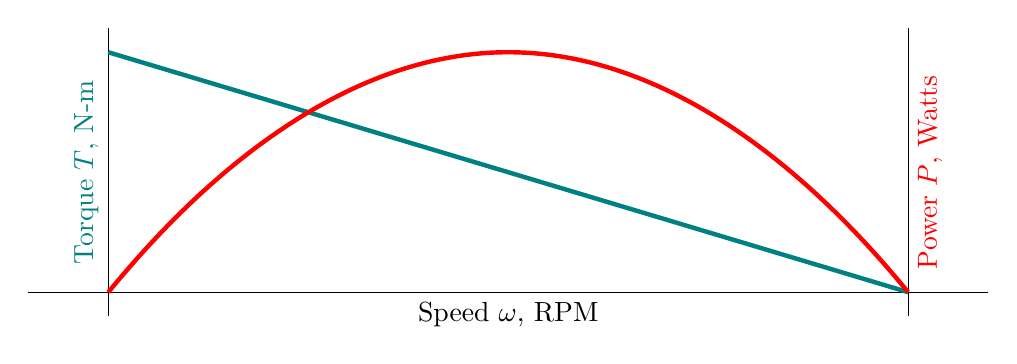
\begin{tikzpicture}[x=4.0in,y=1.2in]
  %\fill[lightgray] (1.0,0)--(0,1.0)--(0,0)--cycle;
  \draw[black] (-0.1,0)--(1.1,0) node[pos=0.5,below]{Speed $\omega$, RPM};
  \draw[black] (0,-0.1)--(0,1.1) node[pos=0.5,above,rotate=90,teal]{Torque $T$, N-m};
  \draw[black] (1,-0.1)--(1,1.1) node[pos=0.5,below,rotate=90,red]{Power $P$, Watts};

  \draw[teal, ultra thick] (1.0,0)--(0,1.0);
  \draw[red, ultra thick] (0,0) parabola bend (0.5,1.0) (1.0,0.0) ;
  
  % TODO: Peak power
\end{tikzpicture}
\caption{Power forms a parabolic curve with speed.}
\end{figure}

From this we can see that the peak power is produced at half of free speed. This is also half of torque.

Current ($I$) is how much electricity is drawn. It varies proportionally to torque, so

\begin{align} \label{eq:motor_current_curve}
  I = C T \nonumber \\
  I = C T_{stall} \frac{\omega_{free}-\omega}{\omega_{free}}
\end{align}

\begin{figure}[H] \centering
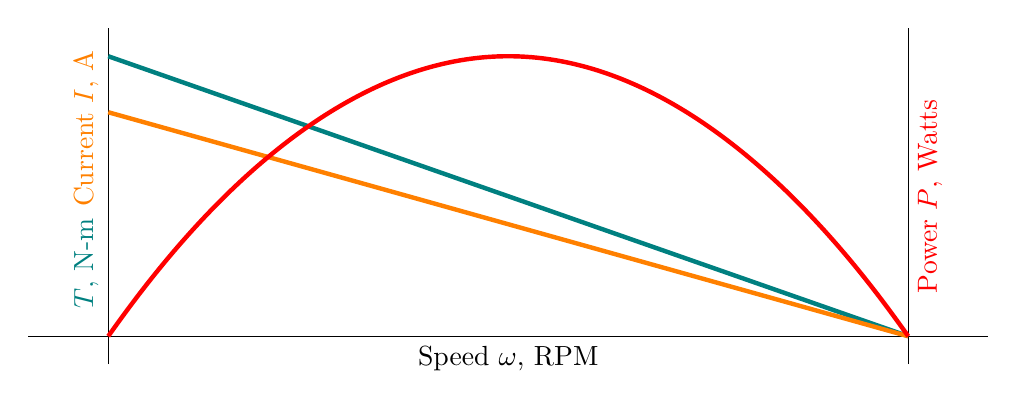
\begin{tikzpicture}[x=4.0in,y=1.4in]
  %\fill[lightgray] (1.0,0)--(0,1.0)--(0,0)--cycle;
  \draw[black] (-0.1,0)--(1.1,0) node[pos=0.5,below]{Speed $\omega$, RPM};
  \draw[black] (0,-0.1)--(0,1.1) node[pos=0.3,above,rotate=90,teal]{$T$, N-m} node[pos=0.7,above,rotate=90,orange]{Current $I$, A};
  \draw[black] (1,-0.1)--(1,1.1) node[pos=0.5,below,rotate=90,red]{Power $P$, Watts};

  \draw[teal, ultra thick] (1.0,0)--(0,1.0);
  \draw[orange, ultra thick] (1.0,0)--(0,0.8);
  \draw[red, ultra thick] (0,0) parabola bend (0.5,1.0) (1.0,0.0) ;
  
  % TODO: Label stall current
\end{tikzpicture}
\caption{Current varies with torque.}
\end{figure}

Efficiency ($\eta$) is a ratio of how much mechanical energy is produced per electrical energy spent.

\begin{equation} \label{eq:motor_efficiency_curve}
  \eta = \frac{P_{mech}}{P_{elec}} = \frac{T-M_{friction} \omega}{V I}
  = \frac{[T_{stall} \ \frac{(\omega_{free}-\omega)}{\omega_{free}} - M_f] \omega}{V\ C\ T_{stall} \frac{(\omega_{free}-\omega)}{\omega_{free}}} \nonumber
\end{equation}

Indeed an ugly equation, let's just plot it with some semi-realistic values.

\begin{figure}[H] \centering
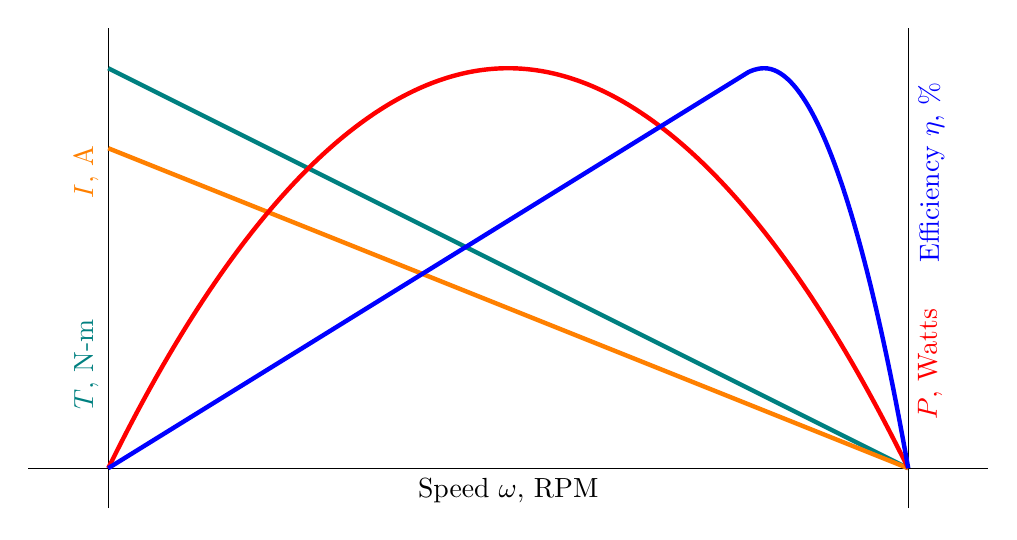
\begin{tikzpicture}[x=4.0in,y=2.0in]
  %\fill[lightgray] (1.0,0)--(0,1.0)--(0,0)--cycle;
  \draw[black] (-0.1,0)--(1.1,0) node[pos=0.5,below]{Speed $\omega$, RPM};
  \draw[black] (0,-0.1)--(0,1.1) node[pos=0.3,above,rotate=90,teal]{$T$, N-m}
  node[pos=0.7,above,rotate=90,orange]{$I$, A};
  \draw[black] (1,-0.1)--(1,1.1) node[pos=0.3,below,rotate=90,red]{$P$, Watts}
  node[pos=0.7,below,rotate=90,blue]{Efficiency $\eta$, \%};

  \draw[teal, ultra thick] (1.0,0)--(0,1.0);
  \draw[orange, ultra thick] (1.0,0)--(0,0.8);
  \draw[red, ultra thick] (0,0) parabola bend (0.5,1.0) (1.0,0.0) ;
  \draw[blue, ultra thick] (0,0)--(0.8,0.99) parabola bend (0.82,1.0) (1.0,0.0) ;
\end{tikzpicture}
\caption{Complete motor curve.}
\end{figure}

In summary:
\begin{asparaitem}
	\item Motors produce less and less torque as they spin up.
	\item No power is produced when the motor is at maximum speed or maximum torque.
	\item Maximum power is produced at 50\% of maximum speed, which is also at 50\% of maximum torque.
	\item Maximum efficiency occurs somewhere between 75\% and 90\% of free speed.
\end{asparaitem}

\chapter{Pneumatics}
\chapter{Complex Systems}

 {\slshape \scshape ``Complex is better than complicated." - The Zen of Python}
 \\

% Intakes
% Vibe feeders
% Elevators
% Arms
% Claws
% Flywheel-based launcher
% Catapult and punch
% Drivetrains
% Swerve Modules



\chapter{Choosing Gear Ratios}

 {\slshape \scshape ``Power is worthless, if improperly wielded"}
 \\

If we have a motor with a pinion of $N_m$ teeth, mating with a driven gear of $N_d$ teeth, we would achieve a gear ratio of

\begin{align}
  G = \frac{N_d}{N_m} = \frac{\omega_m}{\omega_d} = \frac{T_d}{T_m}
\end{align}

This also works with belts or sprockets and chain (though you may need to keep an eye on the direction of rotation, as gears can reverse the direction of rotation).


\begin{figure}[H] \centering
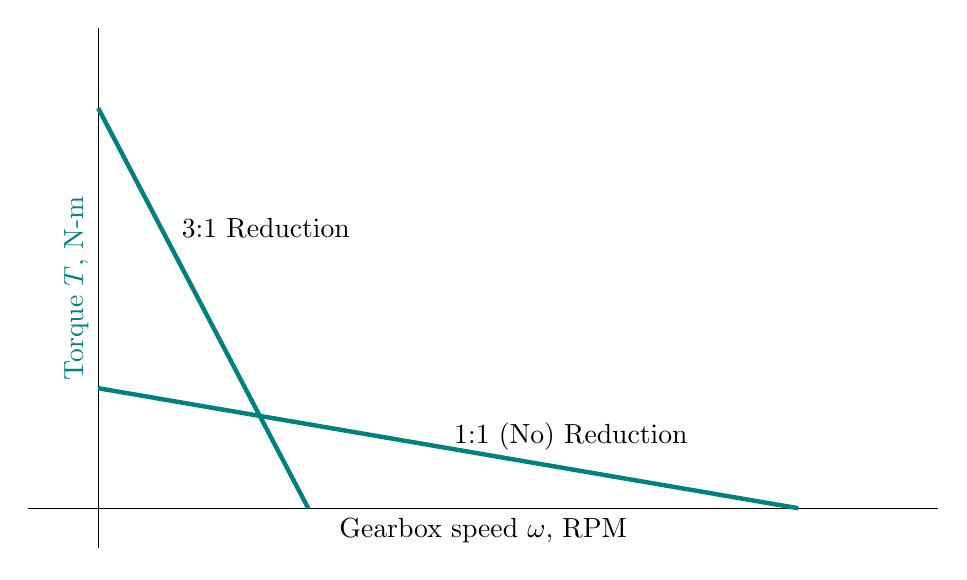
\begin{tikzpicture}[x=3.5in,y=2.0in]
  %\fill[lightgray] (1.0,0)--(0,1.0)--(0,0)--cycle;
  \draw[black] (-0.1,0)--(1.2,0) node[pos=0.5,below]{Gearbox speed $\omega$, RPM};
  \draw[black] (0,-0.1)--(0,1.2) node[pos=0.5,above,rotate=90,teal]{Torque $T$, N-m};

  \draw[teal, ultra thick] (1.0,0)--(0,0.3) node[pos=0.6, right, black]{\ \ \ \ \ \ \ 1:1 (No) Reduction};
  \draw[teal, ultra thick] (0.3,0)--(0,1.0) node[pos=0.7, right, black]{\ 3:1 Reduction};
\end{tikzpicture}
\caption{A 3:1 gear reduction shifts the effective motor curve of a gearbox.}
\end{figure}

The 3:1 ratio reduces maximum speed, but increases the maximum torque. It also changes the RPM at which maximum power and efficiency occur. A gearbox that has too much gear-down:
\begin{asparaitem}
	\item Quickly gets up to its maximum speed and remains there throughout the majority of its action.
	\item Operates beyond the speed necessary for peak efficiency of the motor.
	\item Operates for too long, wasting electrical power.
\end{asparaitem}

Whereas a gearbox that is not geared down enough:
\begin{asparaitem}
	\item Operates below the speed necessary for peak power or efficiency of the motor.
	\item Pulls excessive current, wasting electrical power.
	\item May not even move at all in the first place, lacking the strength to overcome load placed on it.
\end{asparaitem}

But how do we know that we've geared appropriately? We could definitely test all the different ratios, gather all the operating data, and then draw a conclusion... or we could do some pre-emptive math. Don't worry- you don't even need to get your hands too dirty. All of the rough stuff has been done already- you just need to know how to use the design applications to get the answer you want.

But knowing roughly what's going on is important. There's an old joke in engineering,

 {\slshape \scshape ``All data is wrong. But this data, having gone through an incredibly sophisticated computer, is somehow ennobled and none dare question it."}
 
 Which roughly translates to: ``You can't just mash buttons and trust the results".

\section{Developing a Generalized Mechanism Model}

\subsection{The Simple Flywheel Case}

Let's examine a simple case of a motor accelerating a flywheel. This is also (essentially) the same as any system with no friction or gravity-fighting (like an ideal drivetrain).
	
	\begin{figure}[H] \centering
	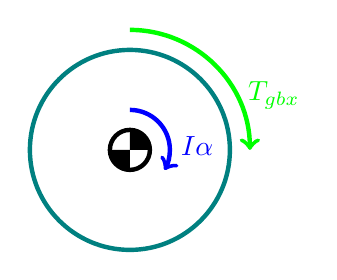
\begin{tikzpicture}[x=1.0in,y=1.0in]
		\draw[ultra thick] (0,0) circle (0.1);
		\fill[black] (0,0.1)--(0,0)--(0.1,0) arc[start angle=0, end angle=90, radius=0.1]--cycle;
		\fill[black] (0,-0.1)--(0,0)--(-0.1,0) arc[start angle=180, end angle=270, radius=0.1]--cycle;
		\draw[ultra thick, teal] (0,0) circle (0.5);
		
		%\draw[ultra thick, red, ->] (0,0.6) arc[start angle=90, end angle=180, radius=0.6] node[pos=0.7,left]{$M_{resist}$};
		\draw[ultra thick, green, ->] (0,0.6) arc[start angle=90, end angle=0, radius=0.6] node[pos=0.7,right]{$T_{gbx}$};
		
		\draw[ultra thick, blue, ->] (0,0.2) arc[start angle=90, end angle=-30, radius=0.2] node[pos=0.7,right]{$I \alpha$};
	\end{tikzpicture}	
	\caption{Free-body diagram of the flywheel}
	\end{figure}	
	
	We can apply conservation of angular momentum to the flywheel.
	\begin{align}
		\sum M &= I \alpha + \cancelto{0 \ \mbox{(no mass transfer)}}{\sum \dot{m}(...)} \\
		T_{gbx} &= I \ \alpha_{wheel}
	\end{align}
	
	This tells us about the rate of acceleration $\alpha$, but what about the velocity $\omega$? 
		
	\begin{align}
		\alpha_{wheel} &= \frac{d \omega_{wheel}}{dt} \\
		\omega_{motor} &= G \omega_{wheel} \\
		G T_{stall} \frac{\omega_{free} - \omega}{\omega_{free}} &= \frac{I}{G} \frac{d \omega}{dt}
	\end{align}
	
		This is a "differential equation" ($\frac{d \omega}{dt}$ and $\omega$ appear in the same equation). These are tricky to solve. \textit{There be dragons ahead. If you don't care to know all the intricate mathy details, skim ahead. I don't blame you.}
		
	\subsection{The Full-Blown Calculus Approach}
	
	We can solve differential equations with calculus!	
	\begin{align}
		\mbox{let }& &B  &= \frac{G^2 T_{stall}}{I} \\
		\mbox{Substitute: }& & B\ \frac{\omega_{free} - \omega}{\omega_{free}} &= \frac{d \omega}{d t} \\
		\mbox{Separate and integrate: }& & \int B\ dt &= \int \frac{\omega_{free}}{\omega_{free} - \omega} d \omega \\
		\mbox{Compute integral (introduces $C$): }& & B t + C &= -\omega_{free}\ ln[\omega_{free} - \omega] \\
		\mbox{Solve for $\omega$: }& & \omega &= \omega_{free} - C\ e^{-\frac{B t}{\omega{max}}} \\
		\mbox{Solve for C with initial condition }& & \omega(0) &= 0 \rightarrow C = \omega_{free} \\
		& &\omega &= \omega_{free}\ [1 - e^{-\frac{G^2\ T_{stall}\ t}{I\ \omega{max}}}] \\
		& &\omega_{gbx} &= \frac{\omega_{free}}{G}\ [1 - e^{-\frac{G^2\ T_{stall}\ t}{I\ \omega{max}}}]
	\end{align}	
	
	If we plot this algebraic solution with some generalized values, we can start to investigate what it really means.	
	
	\begin{figure}[H] \centering
	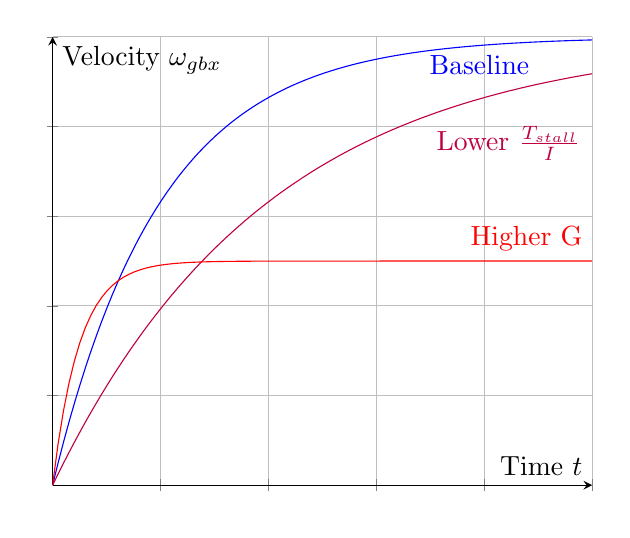
\begin{tikzpicture}[x=3.0in,y=1.5in]
		%\draw[gray] (0,0)--(3,0) node[pos=0.5,below,black]{Time $t$};
		%\draw[gray] (0,0)--(0,2) node[pos=0.5,above,rotate=90,black]{Ang. Velocity $\omega_{gbx}$};
		
		%\draw[red] (0,0)
		
		\begin{axis}[grid=both,
          xmax=5,ymax=1,
          xticklabel=\empty, yticklabel=\empty,
          axis lines=middle,
          restrict y to domain=-7:12,
          xlabel={Time $t$},
          ylabel={Velocity $\omega_{gbx}$}
          ]
		\addplot[blue,domain=0:5,samples=100]  {1*(1-exp(-1^2*x))} node[pos=0.8,below] {Baseline};
		\addplot[purple,domain=0:5,samples=100]  {1*(1-exp(-1^2/2*x))} node[pos=0.7,below right] {Lower $\frac{T_{stall}}{I}$};
		\addplot[red,domain=0:5,samples=100]  {1/2*(1-exp(-2^2*x))} node[above left] {Higher G};
		\end{axis}
	\end{tikzpicture}
	\caption{Flywheel example solution, with different representative parameters}
	\end{figure}
		
	This assumes that there is no constant load, or friction.
	This behavior is generally true, but not exactly true.
	
	\subsection{A Brute-Force Approach}
	We don't need to solve that differential equation using calculus. Or math. We can use basic arithmetic and computers to simulate it! We can do this with a 'numeric differential equation solver', like Newton's Method:
	\begin{equation}
		\frac{d}{dt} f(t) \approx \frac{\Delta f(t)}{\Delta t}
	\end{equation}\begin{equation}
		f(t_{i+1}) = f(t_{i}) + \frac{d}{dt}[f(t_{i})]\ {\Delta t}
	\end{equation}
	
	%TODO: Graphical representation
	
	Another way of putting it... "the next value is the current value, plus the rate of change times the timestep of the simulation". 	We just need to get an expression for the $\frac{d}{dt}f(t)$ we are interested in, and write some code that will repeat this process with a small enough $\Delta t$. This process is sometimes called 'discretization' since we are taking a continuous field of time $t$ and separating it into little $\Delta t$ chunks.	
		
	Let's go back to our flywheel example, and add resistance $M_{resist}$ to it. This $M_{resist}$ can be anything- it can represent friction, air resistance, a spring, you name it! The numeric simulation approach makes this trivial.
	
	\begin{figure}[H] \centering
	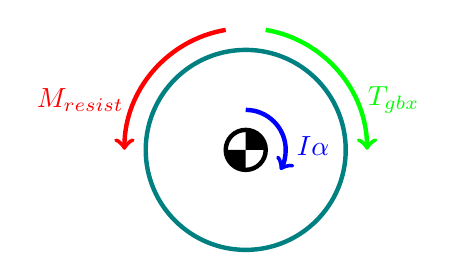
\begin{tikzpicture}[x=1.0in,y=1.0in]
		\draw[ultra thick] (0,0) circle (0.1);
		\fill[black] (0,0.1)--(0,0)--(0.1,0) arc[start angle=0, end angle=90, radius=0.1]--cycle;
		\fill[black] (0,-0.1)--(0,0)--(-0.1,0) arc[start angle=180, end angle=270, radius=0.1]--cycle;
		\draw[ultra thick, teal] (0,0) circle (0.5);
		
		\draw[ultra thick, red, ->] (-0.1,0.6) arc[start angle=99.6, end angle=180, radius=0.608] node[pos=0.7,left]{$M_{resist}$};
		\draw[ultra thick, green, ->] (0.1,0.6) arc[start angle=80.4, end angle=0, radius=0.608] node[pos=0.7,right]{$T_{gbx}$};
		
		\draw[ultra thick, blue, ->] (0,0.2) arc[start angle=90, end angle=-30, radius=0.2] node[pos=0.7,right]{$I \alpha$};
	\end{tikzpicture}	
	\caption{Free-body diagram for the flywheel, with additional resistance $M_{resist}$.}
	\end{figure}
	
	We can go through and repeat the same analysis as before.
	\begin{align}
		\sum M &= I \alpha + \cancelto{0 \ \mbox{(no mass transfer)}}{\sum \dot{m}(...)}  \\
		T_{gbx} - M_{resist} &= I \alpha_{wheel} \\
		\alpha_{wheel} &= \frac{d}{dt} \omega_{wheel} \\
	\end{align}
	
We can solve to yield the equations we need to perform Newton's Method:	
	
	\begin{align}
		\frac{d}{dt} \omega_{wheel} &= \frac{T_{gbx} - M_{resist}}{I} \\
		\frac{d}{dt} \theta_{wheel} &= \omega_{wheel}
	\end{align}
	
	My \href{http://thaddeus-maximus.github.io/swissarmyengineer/}{\color{red}\underline{Swiss Army Engineer}} tool contains a Simple Mechanism Calculator you can use to leverage these physics.

	
\section{Using the Simulations: some analysis/optimization examples}

Let's consider an example drivetrain, with 4 NEOs, 8" diameter wheels, weighing about 143 pounds, meeting 30 N of resistive force. We want to go 10 meters. We have two gear ratio options to consider: a 10:1 gearbox, and a 7:1 gearbox. Which should we pick?

Before you look at the plots, go to the simulator and plug in those values, see if you can come up with an answer of which gets to the destination faster.

\clearpage
	
	\begin{figure}[H] \centering
	\includegraphics[width=0.8\textwidth]{imgs/thsae_1.png}
	\caption{Baseline simulation, G = 10, t = 2.03 s}
	\end{figure}
	
	\begin{figure}[H] \centering
	\includegraphics[width=0.8\textwidth]{imgs/thsae_2.png}
	\caption{Alternative simulation, G = 7, t = 1.88 s}
	\end{figure}
	
	It looks like the ratio of 7 will get to our destination faster!
	
	However, maybe this isn't our only concern. Drivetrains are complex mechanisms with many objectives (as we'll discuss later). The G = 10 case has lower current consumption (almost half!) in this maneuver. It has more initial pushing power. It also gets to positions less than 3 meters away faster. There are a lot of tradeoffs!
	
\chapter{Going Forth}

 {\slshape \scshape ``Learn the rules like a pro, so you can break them like an artist." - Pablo Picasso}
 \\


\end{document}
